\documentclass[11pt]{article}
\usepackage[utf8]{inputenc}
\usepackage[T1]{fontenc}
\usepackage{lmodern}
\usepackage[spanish,provide=*]{babel}
\usepackage{amsmath,amsfonts,amssymb,amsthm}
\usepackage[margin=2.2cm]{geometry}
\usepackage{float}
\usepackage{algorithm}
\usepackage{algpseudocode}
\usepackage{graphicx}
\usepackage{booktabs}
\usepackage{multirow}
\usepackage{enumitem}
\usepackage{xcolor}
\usepackage{caption}
\usepackage{xurl}
\usepackage{makecell}
\usepackage[hidelinks]{hyperref}

\graphicspath{{figuras/}{../figuras/}}
\floatname{algorithm}{Algoritmo}
\renewcommand{\algorithmicrequire}{\textbf{Entrada:}}
\renewcommand{\algorithmicensure}{\textbf{Salida:}}
\newtheorem{prop}{Proposición}
\theoremstyle{remark}
\newtheorem*{obs}{Observación}
\captionsetup{font=small,labelfont=bf}
\AtBeginDocument{\renewcommand{\tablename}{Tabla}\renewcommand{\listtablename}{Índice de tablas}}
\setlist{nosep}
\newcommand{\oct}{\operatorname{oct}}

% Generado por experiments/make_tables.py — no editar a mano
\newcommand{\acoGapTemprano}{12.8}
\newcommand{\acoLiderDesde}{600}
\newcommand{\acoLiderHasta}{21\,000}
\newcommand{\acoLsCombos}{8}
\newcommand{\acoLsMejores}{6}
\newcommand{\apGap}{28.6}
\newcommand{\asimMedia}{35.1}
\newcommand{\bnbBestHardGap}{1.57}
\newcommand{\bnbBestHardVal}{817}
\newcommand{\bnbBestMemMax}{68.8}
\newcommand{\bnbDfsHardVal}{830}
\newcommand{\bnbDfsMaxNodos}{11\,755\,520}
\newcommand{\bnbDfsMem}{15}
\newcommand{\bnbHardOpt}{830}
\newcommand{\bnbLimites}{2}
\newcommand{\bnbOk}{99}
\newcommand{\btConNBA}{98}
\newcommand{\btConNBE}{364}
\newcommand{\btConNBI}{1\,194}
\newcommand{\btConNCC}{6\,185}
\newcommand{\btConNCG}{28\,368}
\newcommand{\btConNDA}{134\,936}
\newcommand{\btSinNBA}{488}
\newcommand{\btSinNBE}{4\,710}
\newcommand{\btSinNBI}{34\,900}
\newcommand{\btSinNCC}{373\,896}
\newcommand{\btTodasOk}{1}
\newcommand{\corridasMeta}{1\,120}
\newcommand{\cspDmax}{100}
\newcommand{\cspDoneBtDCI}{5/10}
\newcommand{\cspDoneBtDDA}{2/10}
\newcommand{\cspDoneBtDDC}{1/10}
\newcommand{\cspDoneFcDCI}{6/10}
\newcommand{\cspDoneFcDDA}{6/10}
\newcommand{\cspDoneFcDDC}{2/10}
\newcommand{\cspDoneFcMrvDCI}{5/10}
\newcommand{\cspDoneFcMrvDDA}{3/10}
\newcommand{\cspDoneFcMrvDDC}{1/10}
\newcommand{\cspDoneMacDCI}{6/10}
\newcommand{\cspDoneMacDDA}{5/10}
\newcommand{\cspDoneMacDDC}{2/10}
\newcommand{\cspMemBt}{72}
\newcommand{\cspMemFc}{211}
\newcommand{\cspMemMac}{1\,155}
\newcommand{\cspMemMc}{84}
\newcommand{\cspMemSmallFc}{24}
\newcommand{\cspMemSmallMac}{62}
\newcommand{\cspNodBtDCI}{52\,583}
\newcommand{\cspNodBtDDA}{100\,009}
\newcommand{\cspNodBtDDC}{100\,012}
\newcommand{\cspNodFcDCI}{422}
\newcommand{\cspNodFcDDA}{16\,243}
\newcommand{\cspNodFcDDC}{100\,000}
\newcommand{\cspNodFcMrvDCI}{50\,216}
\newcommand{\cspNodFcMrvDDA}{100\,000}
\newcommand{\cspNodFcMrvDDC}{100\,000}
\newcommand{\cspNodMacDCI}{196}
\newcommand{\cspNodMacDDA}{3\,599}
\newcommand{\cspNodMacDDC}{24\,192}
\newcommand{\cspSoluciones}{1126}
\newcommand{\cspTBt}{10.2}
\newcommand{\cspTBtDCI}{24}
\newcommand{\cspTBtDDA}{44}
\newcommand{\cspTBtDDC}{42}
\newcommand{\cspTFc}{12.0}
\newcommand{\cspTFcDCI}{219}
\newcommand{\cspTFcDDA}{236}
\newcommand{\cspTFcDDC}{577}
\newcommand{\cspTFcMrvDCI}{183}
\newcommand{\cspTFcMrvDDA}{304}
\newcommand{\cspTFcMrvDDC}{390}
\newcommand{\cspTMac}{858.9}
\newcommand{\cspTMacDCI}{1\,946}
\newcommand{\cspTMacDDA}{2\,061}
\newcommand{\cspTMacDDC}{4\,131}
\newcommand{\cspTMc}{21.1}
\newcommand{\cspValidas}{100}
\newcommand{\ebfMax}{1.52}
\newcommand{\ebfMin}{1.11}
\newcommand{\exBbAcoMem}{17.9}
\newcommand{\exBbAcoNodos}{20\,504}
\newcommand{\exBbAcoT}{992}
\newcommand{\exBbMem}{18.2}
\newcommand{\exBbNodos}{22\,702}
\newcommand{\exBbT}{1\,078}
\newcommand{\exBbVmcNodos}{22\,700}
\newcommand{\exBbVmcT}{1\,031}
\newcommand{\exHkMem}{983.6}
\newcommand{\exHkNodos}{49\,152}
\newcommand{\exHkT}{149}
\newcommand{\exTodosOk}{100}
\newcommand{\gaGap}{0.34}
\newcommand{\gaOpt}{55}
\newcommand{\gapAcoKBAA}{9.51}
\newcommand{\gapAcoKBC}{0.08}
\newcommand{\gapAcoKCF}{1.06}
\newcommand{\gapAcoKFA}{3.94}
\newcommand{\gapAcoLsKBAA}{8.62}
\newcommand{\gapAcoLsKBC}{0.10}
\newcommand{\gapAcoLsKCF}{0.07}
\newcommand{\gapAcoLsKFA}{2.22}
\newcommand{\gapGaKBAA}{85.33}
\newcommand{\gapGaKBC}{0.04}
\newcommand{\gapGaKCF}{1.43}
\newcommand{\gapGaKFA}{9.70}
\newcommand{\gapMemKBAA}{24.14}
\newcommand{\gapMemKBC}{0.04}
\newcommand{\gapMemKCF}{0.70}
\newcommand{\gapMemKFA}{4.35}
\newcommand{\gapSaKBAA}{12.73}
\newcommand{\gapSaKBC}{0.00}
\newcommand{\gapSaKCF}{0.16}
\newcommand{\gapSaKFA}{3.81}
\newcommand{\gapTabuKBAA}{11.84}
\newcommand{\gapTabuKBC}{0.00}
\newcommand{\gapTabuKCF}{0.20}
\newcommand{\gapTabuKFA}{3.94}
\newcommand{\gapUcbKBAA}{10.19}
\newcommand{\gapUcbKBC}{0.00}
\newcommand{\gapUcbKCF}{0.11}
\newcommand{\gapUcbKFA}{2.65}
\newcommand{\hCotaMse}{100}
\newcommand{\hCotaQ}{100}
\newcommand{\hExpA}{3\,855}
\newcommand{\hExpMse}{2\,835}
\newcommand{\hExpQ}{2\,389}
\newcommand{\hExpUCS}{5\,979}
\newcommand{\hExpW}{2\,355}
\newcommand{\hFilas}{600\,000}
\newcommand{\hFracMse}{60.8}
\newcommand{\hFracQ}{31.6}
\newcommand{\hGapA}{0.00}
\newcommand{\hGapMaxA}{0.00}
\newcommand{\hGapMaxMse}{10.00}
\newcommand{\hGapMaxQ}{9.20}
\newcommand{\hGapMaxW}{11.30}
\newcommand{\hGapMse}{1.09}
\newcommand{\hGapQ}{0.34}
\newcommand{\hGapW}{0.65}
\newcommand{\hInfA}{0.0}
\newcommand{\hInfMse}{119.7}
\newcommand{\hInfQ}{139.1}
\newcommand{\hInfW}{0.0}
\newcommand{\hMaeMse}{0.020}
\newcommand{\hMaeQ}{0.029}
\newcommand{\hMapas}{300}
\newcommand{\hSobreMse}{55.4}
\newcommand{\hSobreQ}{20.5}
\newcommand{\hTA}{9.5}
\newcommand{\hTMse}{127.0}
\newcommand{\hTQ}{145.4}
\newcommand{\hTW}{6.2}
\newcommand{\hTest}{100}
\newcommand{\hWallMse}{2.885}
\newcommand{\hWallQ}{1.251}
\newcommand{\hWmaxMse}{1.671}
\newcommand{\hWmaxQ}{1.201}
\newcommand{\hWpA}{0.61}
\newcommand{\hitAco}{29}
\newcommand{\hitAcoLs}{46}
\newcommand{\hitGa}{34}
\newcommand{\hitMem}{43}
\newcommand{\hitSa}{48}
\newcommand{\hitTabu}{49}
\newcommand{\hitUcb}{49}
\newcommand{\hospAbiertos}{7\,277}
\newcommand{\hospRegion}{128}
\newcommand{\hospTotal}{7\,596}
\newcommand{\idaAstarNBC}{15}
\newcommand{\idaAstarNBG}{36}
\newcommand{\idaAstarNCA}{54}
\newcommand{\idaAstarNCE}{116}
\newcommand{\idaAstarNCI}{156}
\newcommand{\idaAstarNI}{14}
\newcommand{\idaAstarOkNBC}{10/10}
\newcommand{\idaAstarOkNBG}{10/10}
\newcommand{\idaAstarOkNCA}{10/10}
\newcommand{\idaAstarOkNCE}{10/10}
\newcommand{\idaAstarOkNCI}{10/10}
\newcommand{\idaAstarOkNI}{10/10}
\newcommand{\idaCrA}{10/10}
\newcommand{\idaCrB}{9/10}
\newcommand{\idaCrC}{5/10}
\newcommand{\idaCrD}{1/10}
\newcommand{\idaCrResueltas}{25/40}
\newcommand{\idaCrTTNBC}{58}
\newcommand{\idaCrTTNBG}{219}
\newcommand{\idaCrTTNCA}{536}
\newcommand{\idaCrTTNCE}{4\,573}
\newcommand{\idaCrTTNCI}{11\,976}
\newcommand{\idaCrTTNI}{90}
\newcommand{\idaCrTTOkNBC}{10/10}
\newcommand{\idaCrTTOkNBG}{10/10}
\newcommand{\idaCrTTOkNCA}{10/10}
\newcommand{\idaCrTTOkNCE}{10/10}
\newcommand{\idaCrTTOkNCI}{10/10}
\newcommand{\idaCrTTOkNI}{10/10}
\newcommand{\idaMemAstarNBC}{2.9}
\newcommand{\idaMemAstarNBG}{4.8}
\newcommand{\idaMemAstarNCA}{8.0}
\newcommand{\idaMemAstarNCE}{11.7}
\newcommand{\idaMemAstarNCI}{20.5}
\newcommand{\idaMemAstarNI}{1.7}
\newcommand{\idaMemCrSinTTNBC}{6.6}
\newcommand{\idaMemCrSinTTNBG}{4.5}
\newcommand{\idaMemCrSinTTNCA}{2\,161.4}
\newcommand{\idaMemCrSinTTNCE}{17.7}
\newcommand{\idaMemCrSinTTNCI}{5\,482.0}
\newcommand{\idaMemCrSinTTNI}{8.4}
\newcommand{\idaMemCrTTNBC}{5.0}
\newcommand{\idaMemCrTTNBG}{4.5}
\newcommand{\idaMemCrTTNCA}{19.0}
\newcommand{\idaMemCrTTNCE}{8.0}
\newcommand{\idaMemCrTTNCI}{338.8}
\newcommand{\idaMemCrTTNI}{4.3}
\newcommand{\idaMemSinTTNBC}{1.0}
\newcommand{\idaMemSinTTNBG}{1.1}
\newcommand{\idaMemSinTTNCA}{1.7}
\newcommand{\idaMemSinTTNCE}{1.6}
\newcommand{\idaMemSinTTNCI}{1.9}
\newcommand{\idaMemSinTTNI}{1.1}
\newcommand{\idaMemTTNBC}{1.3}
\newcommand{\idaMemTTNBG}{1.0}
\newcommand{\idaMemTTNCA}{4.9}
\newcommand{\idaMemTTNCE}{2.2}
\newcommand{\idaMemTTNCI}{4.4}
\newcommand{\idaMemTTNI}{1.4}
\newcommand{\idaResueltas}{7/40}
\newcommand{\idaSinTTNBC}{981}
\newcommand{\idaSinTTNBG}{90\,633}
\newcommand{\idaSinTTNCA}{1\,502\,800}
\newcommand{\idaSinTTNCE}{3\,000\,755}
\newcommand{\idaSinTTNCI}{3\,000\,429}
\newcommand{\idaSinTTNI}{3\,483}
\newcommand{\idaSinTTOkNBC}{8/10}
\newcommand{\idaSinTTOkNBG}{6/10}
\newcommand{\idaSinTTOkNCA}{5/10}
\newcommand{\idaSinTTOkNCE}{3/10}
\newcommand{\idaSinTTOkNCI}{3/10}
\newcommand{\idaSinTTOkNI}{10/10}
\newcommand{\idaTTNBC}{557}
\newcommand{\idaTTNBG}{8\,538}
\newcommand{\idaTTNCA}{62\,057}
\newcommand{\idaTTNCE}{1\,797\,543}
\newcommand{\idaTTNCI}{2\,708\,554}
\newcommand{\idaTTNI}{856}
\newcommand{\idaTTOkNBC}{10/10}
\newcommand{\idaTTOkNBG}{10/10}
\newcommand{\idaTTOkNCA}{10/10}
\newcommand{\idaTTOkNCE}{6/10}
\newcommand{\idaTTOkNCI}{4/10}
\newcommand{\idaTTOkNI}{10/10}
\newcommand{\kagDisc}{0}
\newcommand{\kagInst}{10\,000}
\newcommand{\kagMemBest}{8.4}
\newcommand{\kagMemBnb}{8.4}
\newcommand{\kagMemBt}{9.1}
\newcommand{\kagMemDp}{2.8}
\newcommand{\kagMemMitm}{9.0}
\newcommand{\kagNewDisc}{0}
\newcommand{\kagNewInst}{9\,885}
\newcommand{\kagNewPicks}{0}
\newcommand{\kagTBest}{33}
\newcommand{\kagTBnb}{34}
\newcommand{\kagTBt}{31}
\newcommand{\kagTDp}{24}
\newcommand{\kagTMitm}{179}
\newcommand{\kagTestN}{441}
\newcommand{\kagTrain}{1\,933}
\newcommand{\kagVal}{132}
\newcommand{\mejorGapKBAA}{8.62}
\newcommand{\mejorGapKBC}{0.00}
\newcommand{\mejorGapKCF}{0.07}
\newcommand{\mejorGapKFA}{2.22}
\newcommand{\mejorKBAA}{ACO+LS}
\newcommand{\mejorKBC}{SA}
\newcommand{\mejorKCF}{ACO+LS}
\newcommand{\mejorKFA}{ACO+LS}
\newcommand{\memAstarNBAA}{180}
\newcommand{\memAstarNBFA}{448}
\newcommand{\memAstarNCAA}{831}
\newcommand{\memAstarNFA}{59}
\newcommand{\memIdaCrNBAA}{1\,632}
\newcommand{\memIdaCrNBFA}{5\,559}
\newcommand{\memIdaCrNCAA}{6\,805}
\newcommand{\memIdaCrNFA}{1\,849}
\newcommand{\memIdaNBAA}{7}
\newcommand{\memIdaNBFA}{13}
\newcommand{\memIdaNCAA}{11}
\newcommand{\memIdaNFA}{10}
\newcommand{\memMetaAco}{616}
\newcommand{\memMetaGa}{195}
\newcommand{\memMetaSa}{21}
\newcommand{\memMetaTabu}{169}
\newcommand{\memMetaUcb}{36}
\newcommand{\memUcsNBAA}{188}
\newcommand{\memUcsNBFA}{529}
\newcommand{\memUcsNCAA}{984}
\newcommand{\memUcsNFA}{63}
\newcommand{\metaMasBaratas}{0}
\newcommand{\milpKnapT}{65}
\newcommand{\milpMaxT}{357.9}
\newcommand{\mitmBnbMem}{10}
\newcommand{\mitmHolg}{320.2}
\newcommand{\mitmLim}{7/10}
\newcommand{\mitmMem}{74.0}
\newcommand{\mitmMilpCert}{30/60}
\newcommand{\mitmMilpT}{11.6}
\newcommand{\mitmOk}{100}
\newcommand{\mitmT}{100}
\newcommand{\mitmVerif}{44/60}
\newcommand{\mminA}{0.582}
\newcommand{\mminB}{0.581}
\newcommand{\mminC}{0.506}
\newcommand{\mminD}{0.513}
\newcommand{\mminMax}{0.58}
\newcommand{\mminMin}{0.51}
\newcommand{\otrosMejoraFinalMin}{0.94}
\newcommand{\peorGapKBC}{0.10}
\newcommand{\rCotaMse}{100}
\newcommand{\rCotaQ}{100}
\newcommand{\rExpAstarNBAA}{857}
\newcommand{\rExpAstarNBFA}{2\,551}
\newcommand{\rExpAstarNCAA}{5\,966}
\newcommand{\rExpAstarNFA}{451}
\newcommand{\rExpMseNBAA}{653}
\newcommand{\rExpMseNBFA}{2\,357}
\newcommand{\rExpMseNCAA}{16\,187}
\newcommand{\rExpMseNFA}{114}
\newcommand{\rExpQNBAA}{699}
\newcommand{\rExpQNBFA}{3\,382}
\newcommand{\rExpQNCAA}{10\,110}
\newcommand{\rExpQNFA}{126}
\newcommand{\rExpUcsNBAA}{1\,955}
\newcommand{\rExpUcsNBFA}{5\,176}
\newcommand{\rExpUcsNCAA}{10\,729}
\newcommand{\rExpUcsNFA}{841}
\newcommand{\rExpWNBAA}{440}
\newcommand{\rExpWNBFA}{1\,512}
\newcommand{\rExpWNCAA}{3\,878}
\newcommand{\rExpWNFA}{263}
\newcommand{\rGapMse}{2.55}
\newcommand{\rGapQ}{0.19}
\newcommand{\rInfNBAA}{99.3}
\newcommand{\rInfNBFA}{219.9}
\newcommand{\rInfNCAA}{368.9}
\newcommand{\rInfNFA}{28.1}
\newcommand{\rMedAstarNBAA}{412}
\newcommand{\rMedAstarNBFA}{2\,102}
\newcommand{\rMedAstarNCAA}{5\,154}
\newcommand{\rMedAstarNFA}{242}
\newcommand{\rMedMseNBAA}{156}
\newcommand{\rMedMseNBFA}{1\,070}
\newcommand{\rMedMseNCAA}{2\,003}
\newcommand{\rMedMseNFA}{66}
\newcommand{\rReabNBAA}{462}
\newcommand{\rReabNBFA}{1\,894}
\newcommand{\rReabNCAA}{15\,011}
\newcommand{\rReabNFA}{30}
\newcommand{\rTAstarNBAA}{1.3}
\newcommand{\rTAstarNBFA}{4.6}
\newcommand{\rTAstarNCAA}{12.1}
\newcommand{\rTAstarNFA}{0.6}
\newcommand{\rTMseNBAA}{100.5}
\newcommand{\rTMseNBFA}{224.6}
\newcommand{\rTMseNCAA}{391.7}
\newcommand{\rTMseNFA}{28.3}
\newcommand{\rTQNBAA}{103.6}
\newcommand{\rTQNBFA}{247.4}
\newcommand{\rTQNCAA}{401.1}
\newcommand{\rTQNFA}{27.8}
\newcommand{\rTUcsNBAA}{3.1}
\newcommand{\rTUcsNBFA}{9.2}
\newcommand{\rTUcsNCAA}{20.3}
\newcommand{\rTUcsNFA}{1.1}
\newcommand{\rTWNBAA}{0.7}
\newcommand{\rTWNBFA}{2.6}
\newcommand{\rTWNCAA}{8.0}
\newcommand{\rTWNFA}{0.4}
\newcommand{\rWmaxMse}{2.876}
\newcommand{\rWmaxQ}{1.190}
\newcommand{\redAvsUCS}{47.5}
\newcommand{\tAcoLsMax}{0.86}
\newcommand{\ucbIns}{29.4}
\newcommand{\ucbSwap}{23.4}
\newcommand{\ucbTwo}{47.2}
\newcommand{\valCaminosValidos}{2\,506}
\newcommand{\valExpA}{482}
\newcommand{\valExpUCS}{6\,479}
\newcommand{\valIguales}{375}
\newcommand{\valIgualesHolg}{2\,091}
\newcommand{\valMapas}{2\,506}
\newcommand{\valMasCortos}{0}
\newcommand{\valMaxExcHolg}{6.0}
\newcommand{\valMayorHolg}{415}
\newcommand{\valMedExcHolg}{0.84}
\newcommand{\valMedRatio}{3.1}
\newcommand{\valMenorHolg}{0}
\newcommand{\valObst}{21.2}
\newcommand{\valPctHolg}{83.4}


\title{\textbf{Análisis y Diseño de Algoritmos Avanzados}\\[0.2cm]
\large Capítulo 5 --- Problema 1: Flota de drones para respuesta a desastres}
\author{Carlos Emiliano Nava Flores \quad A00842650\\
Luis Enrique Castillo Carrillo \quad A00842390\\[0.15cm]
Departamento de Ciencias Computacionales}
\date{8 de noviembre de 2026}

\begin{document}
\maketitle

\begin{abstract}
\noindent
Tras un sismo, una flota de drones lleva kits médicos desde un depósito a clínicas de campo.
La ciudad se modela como un grafo dirigido sobre una rejilla $N\times N$ con zonas de exclusión
aérea y viento, de modo que $c(u,v)\neq c(v,u)$ (asimetría media de \asimMedia\,\% en las matrices
de costos). Se implementaron y compararon, en Python, cuatro bloques: (i) rutas con UCS, A*, IDA*
(clásico e IDA*-CR) con la heurística octil$\times$costo mínimo, cuya admisibilidad y consistencia se
demuestran, y una heurística aprendida entrenada en mapas del \emph{2D Path Planning Dataset};
(ii) carga útil con backtracking por máscaras de bits, ramificación y acotamiento (B\&B) con cota
fraccional y \emph{meet-in-the-middle} (MITM), validados contra las \kagInst{} instancias del
\emph{Knapsack Problem Data} (\kagDisc{} discrepancias); (iii) asignación de plataformas y turnos
como CSP con forward checking, AC-3 y MRV/LCV; y (iv) el orden de visita como TSP asimétrico,
resuelto exactamente con B\&B (cota MST) y Held--Karp para $K\le 12$, y con recocido simulado,
búsqueda tabú, GA con OX, ACO (MMAS), una hiperheurística UCB y dos híbridos para
$K\in\{12,25,50,100\}$ y $N\in\{50,100,150,200\}$, con 10 semillas y el óptimo exacto (HiGHS con
cortes DFJ) como referencia. Para los puntos extra se agregan un panel interactivo, la heurística
aprendida con verificación empírica de la cota $w\cdot C^*$ y tres híbridos búsqueda--bioinspirados.
\end{abstract}

\tableofcontents

%=====================================================================
\section{Modelo del problema}
%=====================================================================

\subsection{La ciudad como grafo dirigido}
La ciudad es una rejilla $N\times N$. Cada celda libre es un vértice; las celdas bloqueadas son
zonas de exclusión aérea (edificios colapsados, humo, helicópteros de rescate). Un dron puede
moverse a sus 8 vecinas; no se permiten diagonales que ``corten esquina'' junto a una celda
bloqueada. El viento es un campo suave $\mathbf w:\text{celdas}\to\mathbb R^2$ con
$\|\mathbf w\|\le 1$: un viento dominante de dirección aleatoria más una turbulencia (ruido blanco
filtrado con una gaussiana). El costo de la arista $u\to v$ es
\begin{equation}\label{eq:costo}
  c(u,v)=\ell(u,v)\,\bigl(1-\alpha\,\langle \bar{\mathbf w}(u,v),\hat{\mathbf d}(u,v)\rangle\bigr),
  \qquad \bar{\mathbf w}=\tfrac12(\mathbf w(u)+\mathbf w(v)),
\end{equation}
donde $\ell\in\{1,\sqrt2\}$ es la longitud del movimiento, $\hat{\mathbf d}$ su dirección unitaria y
$\alpha=0.5$. Con viento a favor el costo baja y con viento en contra sube, así que
$c(u,v)-c(v,u)=-2\alpha\,\ell\,\langle\bar{\mathbf w},\hat{\mathbf d}\rangle\neq0$ en general. El
multiplicador queda en $[1-\alpha,1+\alpha]=[0.5,1.5]$. Definimos el \emph{costo mínimo por unidad}
\[
  m_{\min}=\min_{(u,v)\in E}\frac{c(u,v)}{\ell(u,v)}>0 ,
\]
que se calcula exactamente al construir el grafo. En las ciudades de prueba vale \mminA, \mminB,
\mminC{} y \mminD{} para $N=50$, 100, 150 y 200.

\subsection{Heurística octil por costo mínimo}
Sea $\oct(n,g)=\Delta_{\max}+(\sqrt2-1)\Delta_{\min}$ con $\Delta_{\max},\Delta_{\min}$ el mayor y el
menor de $|r_n-r_g|$ y $|c_n-c_g|$. La heurística pedida es
\begin{equation}\label{eq:h}
  h(n)=m_{\min}\cdot \oct(n,g).
\end{equation}

\begin{prop}\label{prop:h}
$h$ es consistente y admisible en el grafo dirigido de~\eqref{eq:costo}.
\end{prop}
\begin{proof}
\emph{Consistencia.} La distancia octil es la distancia de camino más corto en la rejilla
8-conexa sin obstáculos, luego cumple la desigualdad del triángulo; además el movimiento $u\to v$
tiene longitud octil exactamente $\ell(u,v)$. Por tanto $\oct(u,g)\le \ell(u,v)+\oct(v,g)$.
Multiplicando por $m_{\min}>0$ y usando $m_{\min}\,\ell(u,v)\le c(u,v)$ (definición de $m_{\min}$):
$h(u)\le m_{\min}\ell(u,v)+h(v)\le c(u,v)+h(v)$ para toda arista. \emph{Admisibilidad.} Sea
$n=v_0,\dots,v_k=g$ un camino óptimo. Sumando la consistencia a lo largo del camino,
$h(n)\le\sum_i c(v_i,v_{i+1})+h(g)=h^*(n)$ porque $h(g)=0$.
\end{proof}

\begin{obs}
Los obstáculos sólo pueden alargar los caminos, así que la prueba no depende de ellos. El precio de
la garantía es que $h$ es débil cuando el viento es fuerte: con $m_{\min}$ entre 0.5 y 0.6, en los mapas
de prueba el máximo de $h/h^*$ sobre el camino óptimo fue en promedio \hWpA. Eso motiva la heurística
aprendida (sección~\ref{sec:aprendida}).
\end{obs}

\subsection{Escenario integrado}
El depósito y las clínicas son hospitales reales de la zona de Los Ángeles
(\S\ref{sec:datos}): se proyectan $(\text{lat},\text{lon})$ a la rejilla y cada uno se mueve a la
celda libre más cercana de la componente conexa mayor, sin repetir celdas. El depósito es el
LAC+USC Medical Center. Las zonas de exclusión se generan con el mismo procedimiento que los mapas
del dataset de Kaggle (ruido binario y apertura morfológica, \S\ref{sec:datos}), a $100\times100$ y
reescaladas a $N\times N$ para que el área bloqueada no dependa de $N$. La
Figura~\ref{fig:mision} muestra la misión de ejemplo con $N=100$ y $K=25$.

\begin{figure}[t]
\centering
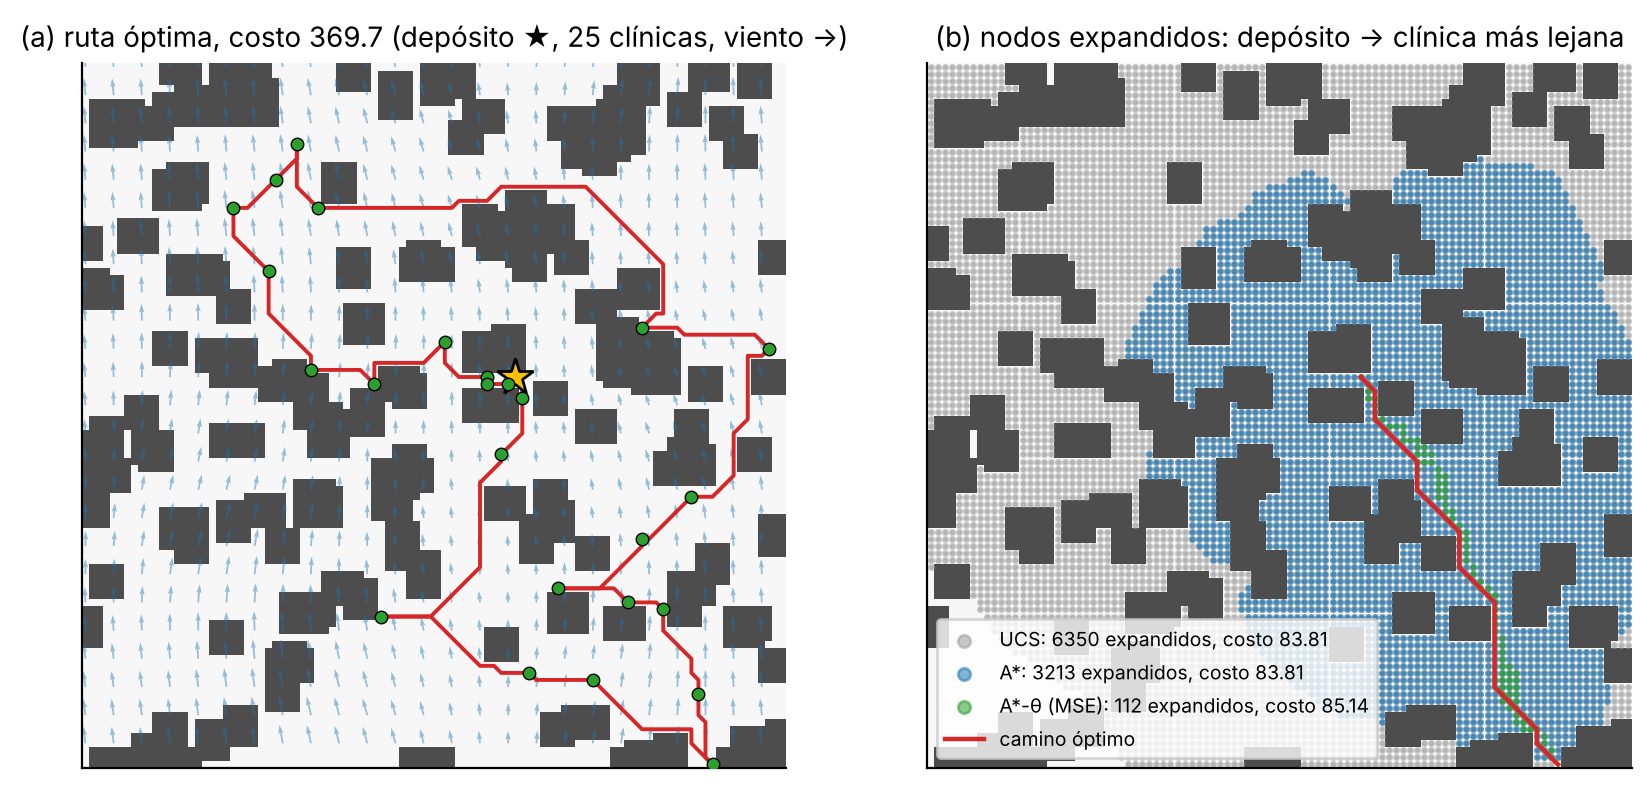
\includegraphics[width=\linewidth]{fig_mision.png}
\caption{Misión de ejemplo ($N=100$, $K=25$). (a) Zonas de exclusión (gris), viento (flechas),
depósito (estrella) y la ruta óptima del ATSP dibujada como los caminos de A* de cada tramo.
(b) Nodos expandidos por UCS, A* y A* con la heurística aprendida en la consulta del depósito a la
clínica más costosa.}
\label{fig:mision}
\end{figure}

%=====================================================================
\section{Datasets}\label{sec:datos}
%=====================================================================

Los mapas son los archivos originales del \emph{2D Path Planning Dataset} de Kaggle. Para los otros
dos datasets se usaron copias públicas: una copia exacta del archivo de la mochila y una base de hospitales con la misma
fuente (HIFLD). La Tabla~\ref{tab:datos} documenta cada una. El código también lee el CSV original de
hospitales de Kaggle si se coloca en \texttt{datos/}.

\begin{table}[H]
\centering\small
\caption{Datasets usados. Fechas de descarga: 8 de noviembre de 2026 (mapas) y 3 de noviembre de
2026 (hospitales y mochila).}\label{tab:datos}
\begin{tabular}{p{2.7cm}p{5.3cm}p{7.6cm}}
\toprule
Dataset (Kaggle) & Fuente usada & Preprocesamiento \\
\midrule
2D Path Planning Dataset\newline
\scriptsize\url{kaggle.com/datasets/dcaffo/2dpathplanningdataset} &
Archivo original de Kaggle (\texttt{archive.zip}, 646\,MB): carpetas \texttt{train},
\texttt{validation} y \texttt{test} con un \texttt{.pt} (objeto \texttt{MapSample} de PyTorch) por
mapa &
Se tomó una muestra sistemática (uno de cada $k$ archivos del zip) de
\valMapas{} mapas $100\times100$: \kagTrain{} de \texttt{train}, \kagVal{} de \texttt{validation} y
\kagTestN{} de \texttt{test}. Los \texttt{.pt} se leen sin PyTorch, reconstruyendo cada tensor
(\texttt{map}, \texttt{start}, \texttt{goal}, \texttt{path}) desde el zip. Celda $=1$ es obstáculo; el
camino de referencia es el de D* Lite. Se entrena con \hMapas{} mapas de \texttt{train} y se prueba
con \hTest{} de \texttt{test} (muestras con semilla 0). \\
\addlinespace
US Hospital Locations\newline
\scriptsize\url{kaggle.com/datasets/andrewmvd/us-hospital-locations} &
CovidCareMap, \scriptsize\url{github.com/covidcaremap/covid19-healthsystemcapacity}
({\scriptsize\path{us_healthcare_capacity-facility-CovidCareMap.csv}}); cada fila trae su \texttt{HIFLD-ID}, la
misma fuente HIFLD del dataset de Kaggle &
Filtro a la caja $33.70\le\text{lat}\le34.35$, $-118.70\le\text{lon}\le-117.90$ (127 hospitales),
sin coordenadas repetidas; proyección lineal a la rejilla y ajuste a la celda libre más cercana. \\
\addlinespace
Knapsack Problem Data\newline
\scriptsize\url{kaggle.com/datasets/warcoder/knapsack-problem} &
Copia exacta \texttt{knapsack\_5\_items.csv} en \scriptsize\url{github.com/Kralog2/Tarea3IA}
(SHA-256 \texttt{55b98b9d\ldots044c}) &
10\,000 instancias de 5 kits (peso, precio, capacidad, solución óptima). Se parsean los arreglos en
texto; 121 filas con \emph{Best picks} vacío (ningún kit cabe, \emph{Best price}$=0$) se toman como
el vector cero. Los $50\,000$ kits forman el \emph{pool} del que se muestrean instancias de
$n=10$ a $120$. \\
\bottomrule
\end{tabular}
\end{table}

%=====================================================================
\section{Rutas: UCS, A* e IDA*}
%=====================================================================

\subsection{Algoritmos}
\textbf{UCS} es Dijkstra con prueba de meta al expandir. \textbf{A*} usa $f=g+h$ con la
heurística~\eqref{eq:h}; a igual $f$ prefiere el mayor $g$. Como $h$ es consistente, ningún nodo se
reabre. \textbf{IDA*} hace búsquedas en profundidad con umbral creciente sobre $f$. Se implementaron
dos políticas de umbral:
\begin{itemize}
\item \emph{IDA* clásico} (Korf): el nuevo umbral es el menor $f$ que excedió al anterior. La primera
solución es óptima, pero con costos reales casi cada iteración agrega un solo valor de $f$, y el
número de iteraciones crece con el número de valores distintos de $f$.
\item \emph{IDA*-CR} (Sarkar et al., 1991): el umbral se elige entre los $f$ excedidos para que la
siguiente iteración tenga $\approx$ el doble de nodos. Si en esa iteración aparece una meta, la DFS
sigue como B\&B (poda $f\ge$ mejor costo) hasta agotar la iteración; entonces la solución es óptima,
porque todo nodo de un camino óptimo tiene $f\le C^*\le$ umbral y se visita.
\end{itemize}
En una rejilla hay muchísimos caminos distintos hacia una misma celda (transposiciones), y sin
memoria IDA* los recorre todos. Por eso ambas variantes se probaron con y sin \emph{tabla de
transposición} (TT) por iteración: se poda si se llega a un nodo con $g$ mayor o igual al mejor $g$
visto en esa iteración, lo cual es seguro porque el presupuesto restante sería menor o igual.

El \emph{factor de ramificación efectivo} $b^*$ resuelve $N_{\text{gen}}+1=1+b^*+\dots+(b^*)^d$
(Russell y Norvig), con $N_{\text{gen}}$ los nodos generados sin contar la raíz (la raíz es el 1 del
lado derecho) y $d$ el número de aristas de la solución; se calcula por bisección.

\subsection{Validación con el dataset}
Sin viento y con los costos del dataset (pasos de 1 y $\sqrt2$, cortes de esquina permitidos) se
compararon UCS y A* con los caminos de referencia de D* Lite en los \valMapas{} mapas (obstáculos:
\valObst\,\% del área). Los \valCaminosValidos{} caminos de referencia son caminos válidos de
8-vecindad, pero no son los más cortos del mapa: en mediana miden \valMedRatio\,\% más que el óptimo de
UCS/A*, sólo \valIguales{} coinciden con él y ninguno (\valMasCortos) es más corto. La razón es que el
autor generó el dataset con \texttt{obst\_margin}\,=\,1 (así está en su
\texttt{dataset/ds\_generator.py}): su planificador no pasa por celdas vecinas a un obstáculo, salvo
junto al inicio o la meta, y en efecto ningún camino de referencia lo hace. Con ese mismo modelo
(obstáculos inflados una celda), el costo de A* coincide con el de referencia en \valIgualesHolg{} de los
\valMapas{} mapas (\valPctHolg\,\%). En los \valMayorHolg{} restantes A* encuentra un camino ligeramente
más barato (mediana \valMedExcHolg\,\%, máximo \valMaxExcHolg\,\%), y en ninguno uno más caro
(\valMenorHolg). El D* Lite publicado por el autor, corrido sobre varios de esos mapas, también da
nuestro costo y no el del dataset, así que la diferencia viene de la versión del planificador con que
se generó (su código intenta primero una implementación en C++ que no está en el repositorio), no de
UCS/A*. UCS y A* coincidieron siempre entre sí; en promedio A* expandió \valExpA{} nodos contra
\valExpUCS{} de UCS.

\subsection{Resultados en las ciudades}
Para cada $N\in\{50,100,150,200\}$ se hicieron 20 consultas entre pares de hospitales del
escenario (las mismas para todos los métodos). Las dos variantes de IDA* se corrieron en las
primeras 10, con límite de 15\,s y $4\cdot10^6$ nodos. El costo óptimo $C^*$ se obtiene con un
Dijkstra independiente (SciPy). La Tabla~\ref{tab:busqueda} y la Figura~\ref{fig:busqueda} resumen los
resultados.

\begin{table}[t]
\centering\scriptsize
\caption{Búsqueda de rutas en las ciudades (media $\pm$ d.e. sobre las consultas resueltas;
memoria pico de Python medida con \texttt{tracemalloc} en las 3 primeras consultas, para las que llegan al
límite repitiendo la búsqueda hasta el mismo número de nodos; brecha respecto a $C^*$).}
\label{tab:busqueda}
\setlength{\tabcolsep}{4pt}
\begin{tabular}{llrrrrrr}
\toprule
$N$ & método & resueltas & nodos expandidos & $b^*$ & tiempo [ms] & mem. [KiB] & brecha [\%] \\
\midrule
\multirow{7}{*}{50} & UCS & 20/20 & 1\,000 $\pm$ 563 & 1.391 & 2.6 $\pm$ 2.5 & 49 & 0.00 \\
 & A* & 20/20 & 444 $\pm$ 385 & 1.277 & 0.7 $\pm$ 1.1 & 45 & 0.00 \\
 & IDA*-CR & 10/10 & 297\,738 $\pm$ 463\,959 & 1.898 & 804.8 $\pm$ 1\,235.1 & 156 & 0.00 \\
 & IDA* & 3/10 & 217\,203 $\pm$ 201\,565 & 3.068 & 554.4 $\pm$ 518.8 & 6 & 0.00 \\
 & WA* (w=1.5) & 20/20 & 259 $\pm$ 243 & 1.241 & 0.3 $\pm$ 0.3 & 44 & 0.04 \\
 & A*-$\theta$ (MSE) & 20/20 & 157 $\pm$ 138 & 1.207 & 41.4 $\pm$ 3.5 & 1\,552 & 1.06 \\
 & A*-$\theta$ (q=0.2) & 20/20 & 151 $\pm$ 133 & 1.216 & 41.0 $\pm$ 0.5 & 1\,552 & 0.02 \\
\midrule
\multirow{7}{*}{100} & UCS & 20/20 & 2\,466 $\pm$ 1\,736 & 1.337 & 4.5 $\pm$ 3.2 & 209 & 0.00 \\
 & A* & 20/20 & 949 $\pm$ 868 & 1.229 & 1.6 $\pm$ 1.5 & 191 & 0.00 \\
 & IDA*-CR & 8/10 & 464\,107 $\pm$ 1\,194\,830 & 1.886 & 1\,293.7 $\pm$ 3\,312.0 & 2\,675 & 0.00 \\
 & IDA* & 3/10 & 60\,016 $\pm$ 90\,031 & 2.895 & 142.5 $\pm$ 213.6 & 13 & 0.00 \\
 & WA* (w=1.5) & 20/20 & 473 $\pm$ 522 & 1.191 & 0.7 $\pm$ 0.9 & 185 & 0.22 \\
 & A*-$\theta$ (MSE) & 20/20 & 740 $\pm$ 1\,637 & 1.167 & 115.0 $\pm$ 26.0 & 6\,005 & 3.02 \\
 & A*-$\theta$ (q=0.2) & 20/20 & 445 $\pm$ 673 & 1.174 & 119.2 $\pm$ 28.1 & 6\,005 & 0.24 \\
\midrule
\multirow{7}{*}{150} & UCS & 20/20 & 6\,313 $\pm$ 3\,440 & 1.121 & 11.5 $\pm$ 6.4 & 486 & 0.00 \\
 & A* & 20/20 & 3\,064 $\pm$ 2\,637 & 1.103 & 5.3 $\pm$ 4.7 & 444 & 0.00 \\
 & IDA*-CR & 3/10 & 1\,211\,171 $\pm$ 500\,213 & 1.356 & 3\,876.1 $\pm$ 1\,488.0 & 5\,014 & 0.00 \\
 & IDA* & 0/10 & -- & -- & -- & 16 & -- \\
 & WA* (w=1.5) & 20/20 & 1\,920 $\pm$ 2\,021 & 1.091 & 3.6 $\pm$ 4.1 & 430 & 0.17 \\
 & A*-$\theta$ (MSE) & 20/20 & 5\,927 $\pm$ 11\,635 & 1.088 & 317.4 $\pm$ 49.0 & 13\,427 & 2.66 \\
 & A*-$\theta$ (q=0.2) & 20/20 & 4\,487 $\pm$ 7\,690 & 1.088 & 318.7 $\pm$ 56.3 & 13\,427 & 0.35 \\
\midrule
\multirow{7}{*}{200} & UCS & 20/20 & 9\,372 $\pm$ 5\,247 & 1.105 & 19.1 $\pm$ 11.0 & 914 & 0.00 \\
 & A* & 20/20 & 4\,766 $\pm$ 3\,363 & 1.086 & 9.7 $\pm$ 7.4 & 820 & 0.00 \\
 & IDA*-CR & 2/10 & 1\,332\,718 $\pm$ 1\,860\,151 & 1.501 & 4\,196.8 $\pm$ 5\,863.1 & 6\,589 & 0.00 \\
 & IDA* & 0/10 & -- & -- & -- & 12 & -- \\
 & WA* (w=1.5) & 20/20 & 3\,200 $\pm$ 2\,482 & 1.080 & 6.6 $\pm$ 5.5 & 790 & 0.26 \\
 & A*-$\theta$ (MSE) & 20/20 & 17\,438 $\pm$ 21\,605 & 1.075 & 479.0 $\pm$ 114.5 & 23\,818 & 4.78 \\
 & A*-$\theta$ (q=0.2) & 20/20 & 12\,855 $\pm$ 26\,687 & 1.072 & 470.1 $\pm$ 89.3 & 23\,818 & 0.24 \\
\bottomrule
\end{tabular}

\end{table}

\begin{figure}[t]
\centering
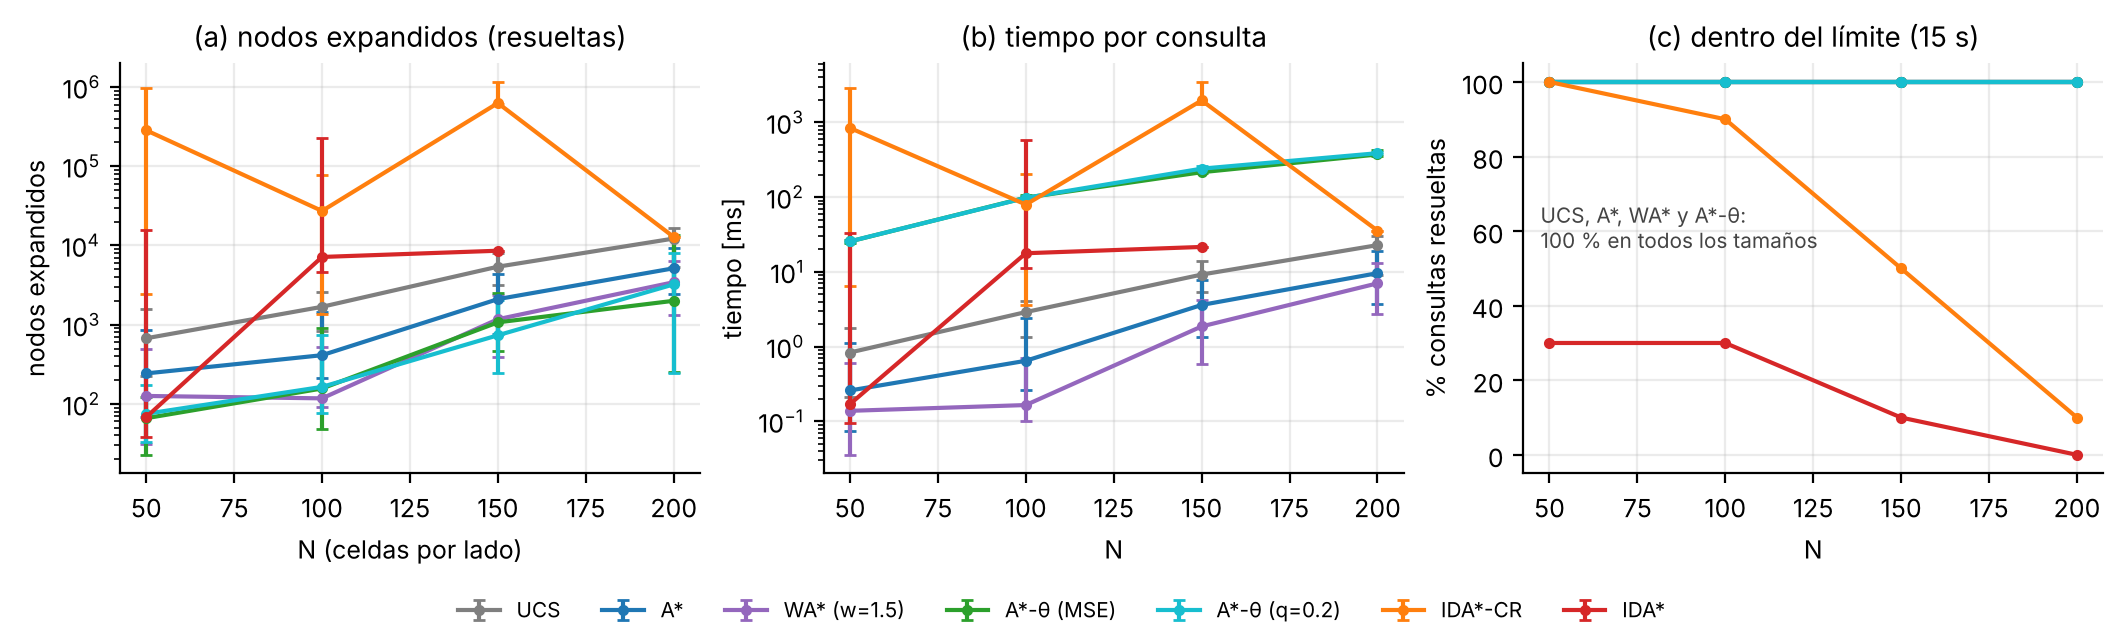
\includegraphics[width=\linewidth]{fig_busqueda_escala.png}
\caption{Escalamiento de la búsqueda de rutas con el tamaño de la rejilla (mediana y rango
intercuartil de las consultas resueltas; 20 consultas por tamaño, 10 para IDA*).}
\label{fig:busqueda}
\end{figure}

Lo principal:
\begin{itemize}
\item UCS, A* e IDA*-CR (cuando termina) son óptimos en todas las consultas. A* expande
\redAvsUCS\,\% menos nodos que UCS en total. La ganancia es moderada porque $h$ es conservadora
($m_{\min}$ entre 0.51 y 0.58).
\item El $b^*$ de UCS y A* queda entre 1.2 y 1.4 porque $d$ es grande (del orden de $N$); sirve más
para comparar métodos en una misma consulta que entre tamaños. El de IDA* es mucho mayor porque
cuenta todos los nodos generados en todas las iteraciones.
\item IDA* resolvió \idaCrResueltas{} consultas con la política CR y sólo \idaResueltas{} con la
clásica. Aun con TT, IDA* re-expande muchas veces los nodos a los que llega primero por un camino
malo, y su tiempo es órdenes de magnitud mayor que el de A*. Su ventaja teórica (memoria $O(d)$) sólo
existe sin TT, y sin TT el número de caminos explota (Figura~\ref{fig:ida}): con $N=24$ IDA* sin TT
resolvió \idaSinTTOkNCE{} consultas, contra \idaCrTTOkNCE{} de IDA*-CR con TT, mientras A* expande
una mediana de \idaAstarNCE{} nodos. En memoria, en cambio, IDA* sin TT sí cumple su promesa: con
$N=24$ su pico fue de \idaMemSinTTNCE\,KiB (sólo la pila), contra \idaMemAstarNCE\,KiB de A* y
\idaMemCrTTNCE\,KiB de IDA*-CR con TT (medianas de 3 consultas).
\end{itemize}

\begin{figure}[t]
\centering
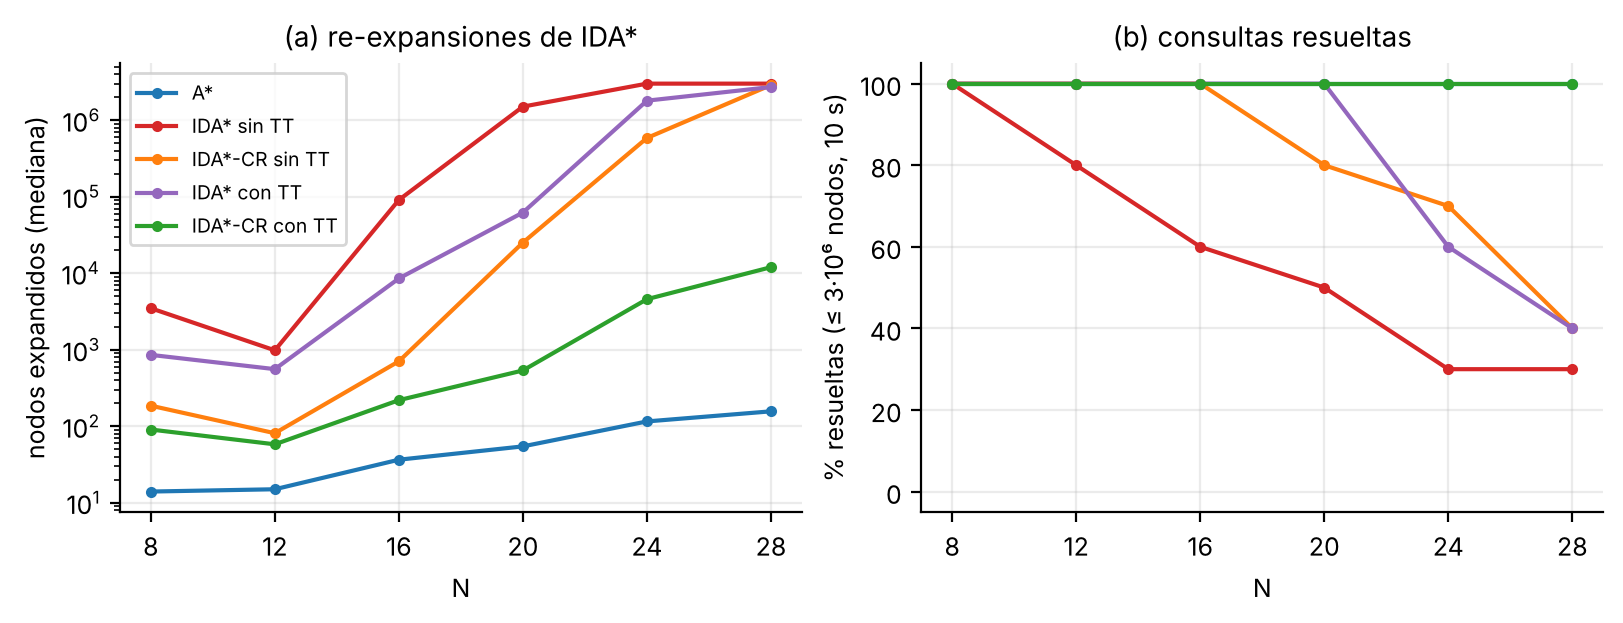
\includegraphics[width=0.85\linewidth]{fig_ida_pequenas.png}
\caption{IDA* en rejillas pequeñas con viento (10 consultas por tamaño, límite de $3\cdot10^6$ nodos
o 10\,s). Sin tabla de transposición, el número de caminos que recorre crece exponencialmente.}
\label{fig:ida}
\end{figure}

\subsection{Heurística aprendida}\label{sec:aprendida}
\paragraph{Modelo.} Se aprende el cociente $r(n)=h^*(n)/\oct(n,g)$ y se usa
$h_\theta(n)=\oct(n,g)\,\hat r(n)$, con $h_\theta(g)=0$. Los rasgos se calculan para todas las
celdas a la vez: distancias octil y euclidiana, fracción de celdas bloqueadas y número de cruces de
obstáculo en 16 muestras del segmento $n\to g$, viento proyectado sobre ese segmento, densidad local
de obstáculos alrededor de $n$ y de $g$, $|\Delta r|$, $|\Delta c|$, densidad global y $m_{\min}$.
El objetivo $h^*$ se obtiene con un Dijkstra en el grafo inverso desde la meta.

\paragraph{Entrenamiento.} En \hMapas{} mapas de la carpeta \texttt{train} del dataset, cada uno con un
viento aleatorio, y la meta del camino de referencia, se tomaron 2\,000 celdas por mapa (\hFilas{} filas).
Se entrenaron dos modelos de \emph{gradient boosting} (HistGradientBoosting de scikit-learn):
con pérdida cuadrática (MSE) y con pérdida de cuantil $0.2$, que sesga la predicción hacia abajo.
En el 10\,\% de validación el error absoluto medio de $\hat r$ fue \hMaeMse{} y \hMaeQ{}, y la fracción
de celdas sobreestimadas fue \hSobreMse\,\% y \hSobreQ\,\%.

\paragraph{Garantía cuando sobreestima.} $h_\theta$ no es admisible ni consistente, así que se usa
A* \emph{con reapertura} de nodos.

\begin{prop}\label{prop:w}
Sea $P^*$ un camino óptimo de $s$ a $g$ y $w_P=\max\{1,\max_{n\in P^*}h(n)/h^*(n)\}$. Si A* reabre
nodos cerrados cuando mejora su $g$ y $h(g)=0$, el costo devuelto cumple $C\le w_P\cdot C^*$.
\end{prop}
\begin{proof}
Mientras $g$ no se haya expandido, existe en OPEN un nodo $n'\in P^*$ con $g(n')=g^*(n')$: es el
primer nodo de $P^*$ que no está cerrado con su $g$ óptimo; su predecesor en $P^*$ sí lo está, y al
expandirlo le asignó $g^*(n')$ (con reapertura, aunque $n'$ estuviera cerrado con un $g$ peor).
Entonces $f(n')=g^*(n')+h(n')\le g^*(n')+w_Ph^*(n')\le w_P\,(g^*(n')+h^*(n'))=w_P\,C^*$. Cuando A*
elige $g$, $C=f(g)\le f(n')\le w_P C^*$.
\end{proof}

En cada consulta de prueba se calculó $h^*$ en todo el mapa, $w_P$ sobre el camino óptimo de A* y
también $w_{\text{all}}=\max_n h_\theta/h^*$ sobre todas las celdas. La Tabla~\ref{tab:heur} y la
Figura~\ref{fig:heur} muestran que la cota se cumplió en el \hCotaMse\,\% (MSE) y \hCotaQ\,\% (cuantil)
de los \hTest{} mapas de prueba y en el \rCotaMse\,\%/\rCotaQ\,\% de las consultas en las ciudades.
En los mapas de prueba el modelo MSE llegó a $w_P=\hWmaxMse$ ($w_{\text{all}}$ hasta \hWallMse), con
brecha media de \hGapMse\,\% y máxima de \hGapMaxMse\,\%; el de cuantil, más conservador, tuvo
$w_P\le\hWmaxQ$ y brecha media de \hGapQ\,\% (máxima \hGapMaxQ\,\%). En las ciudades, fuera de la
escala de entrenamiento, $w_P$ llegó a \rWmaxMse{} (MSE) y \rWmaxQ{} (cuantil): la cota se sigue
cumpliendo, pero ya no dice mucho.

\begin{table}[t]
\centering\scriptsize
\caption{Heurística aprendida frente a A* admisible y A* ponderado ($w=1.5$). El tiempo incluye la
inferencia del modelo (\hInfMse\,ms por consulta en promedio en los mapas de prueba); la memoria (pico
de Python en 3 mapas o consultas) incluye la matriz de rasgos de toda la rejilla.}
\label{tab:heur}
\resizebox{\linewidth}{!}{\begin{tabular}{lrrrrrrrrr}
\toprule
método & brecha [\%] & máx. [\%] & óptimas [\%] & expandidos & tiempo [ms] & $\bar w_P$ & $\max w_P$ & cota ok [\%] & mem. [KiB] \\
\midrule
\multicolumn{10}{l}{\emph{mapas de prueba del dataset (100$\times$100)}} \\
UCS & 0.00 & 0.00 & 100 & 5\,979 & 12.4 & -- & -- & 100 & 332 \\
A* & 0.00 & 0.00 & 100 & 3\,855 & 9.5 & -- & -- & 100 & 275 \\
WA* (w=1.5) & 0.65 & 11.30 & 58 & 2\,355 & 6.2 & 1.5 & 1.5 & 100 & 244 \\
A*-$\theta$ (MSE) & 1.09 & 10.00 & 3 & 2\,835 & 127.0 & 1.126 & 1.671 & 100 & 6\,005 \\
A*-$\theta$ (q=0.2) & 0.34 & 9.20 & 11 & 2\,389 & 145.4 & 1.030 & 1.201 & 100 & 6\,005 \\
\midrule
\multicolumn{10}{l}{\emph{ciudades $N\in\{50,\dots,200\}$}} \\
UCS & 0.00 & 0.00 & 100 & 4\,788 & 9.4 & -- & -- & -- & 415 \\
A* & 0.00 & 0.00 & 100 & 2\,306 & 4.3 & -- & -- & -- & 375 \\
WA* (w=1.5) & 0.17 & 3.73 & 72 & 1\,463 & 2.8 & 1.5 & 1.5 & -- & 362 \\
A*-$\theta$ (MSE) & 2.88 & 21.97 & 15 & 6\,065 & 238.2 & 1.424 & 3.532 & 100 & 11\,200 \\
A*-$\theta$ (q=0.2) & 0.21 & 4.94 & 49 & 4\,485 & 237.3 & 1.033 & 1.175 & 100 & 11\,200 \\
\bottomrule
\end{tabular}
}
\end{table}

\begin{figure}[t]
\centering
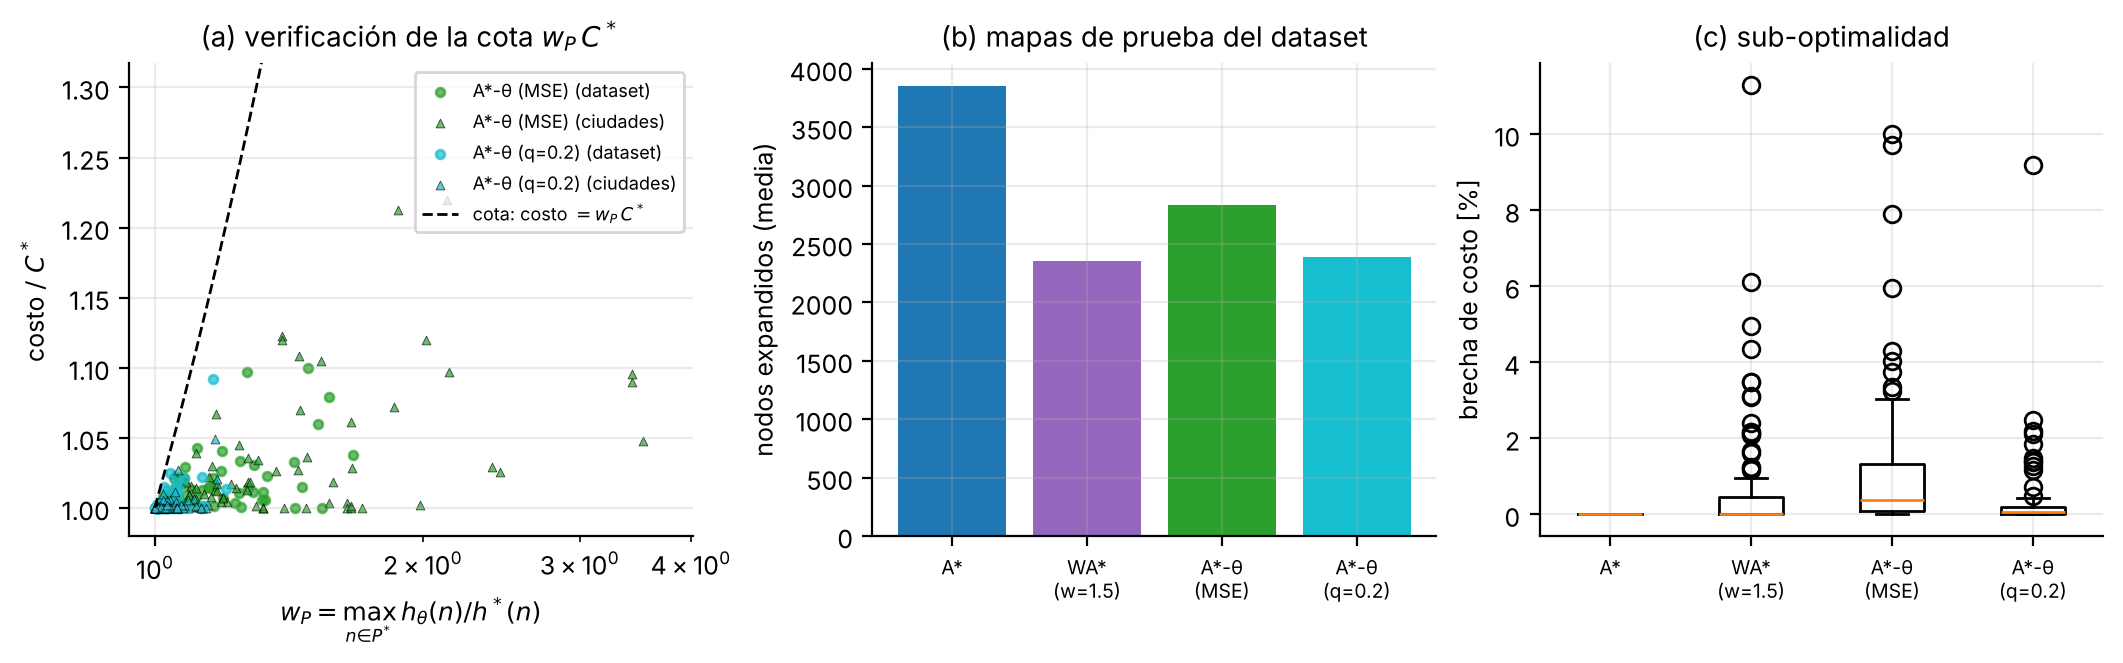
\includegraphics[width=\linewidth]{fig_heuristica.png}
\caption{(a) Todas las consultas quedan bajo la diagonal costo$=w_P C^*$, como predice la
Proposición~\ref{prop:w}. (b) Nodos expandidos y (c) brecha en los mapas de prueba del dataset.}
\label{fig:heur}
\end{figure}

En los mapas de prueba del dataset la heurística aprendida redujo los nodos expandidos respecto a A*
(\hExpMse{} y \hExpQ{} contra \hExpA), pero menos de lo que su error medio sugeriría: sus errores no
son suaves entre celdas vecinas, así que $f$ sube y baja a lo largo de los caminos y A* termina
explorando una banda de nodos alrededor de $C^*$. En las ciudades el efecto depende de la escala. Con
$N=50$ y $N=100$, la escala de los mapas de entrenamiento, A*-$\theta$ (MSE) expandió \rExpMseNFA{} y
\rExpMseNBAA{} nodos contra \rExpAstarNFA{} y \rExpAstarNBAA{} de A* (Figura~\ref{fig:mision}b muestra
un caso). Con $N=200$ expandió en promedio \rExpMseNCAA, más que UCS (\rExpUcsNCAA), y \rReabNCAA{} de esas
expansiones fueron reaperturas; la mediana (\rMedMseNCAA, contra \rMedAstarNCAA{} de A*) muestra que no
falla en todas las consultas, sino que algunas explotan: las distancias salen del rango visto al entrenar con mapas de $100\times100$, los
árboles de decisión no extrapolan y la heurística se vuelve muy inconsistente. Además, calcular $h_\theta$ en toda la rejilla cuesta
\rInfNBAA\,ms con $N=100$ y \rInfNCAA\,ms con $N=200$, más que toda la búsqueda de A*.

A* ponderado con $w=1.5$ expandió menos nodos en todos los tamaños con una cota \emph{demostrable} de
$1.5\,C^*$. La heurística aprendida sólo conviene si su inferencia se amortiza (muchas consultas con la
misma meta), si las consultas se parecen a las de entrenamiento y si se acepta que su $w$ es una
cantidad \emph{medida}, no garantizada.

%=====================================================================
\section{Carga útil de cada dron}
%=====================================================================

Cada dron elige kits $x\in\{0,1\}^n$ para maximizar el valor (prioridad médica) con capacidad $W$ y
pares incompatibles $E$ (por ejemplo, cadena de frío y compresas térmicas):
\[
\max\ \textstyle\sum_i v_ix_i\quad\text{s.a.}\quad\sum_iw_ix_i\le W,\qquad x_i+x_j\le1\ \ \forall(i,j)\in E.
\]
Las instancias se arman con kits del dataset de Kaggle, $W=40\,\%$ del peso total y conflictos
aleatorios con grado medio $1.5$; los kits se ordenan por densidad $v_i/w_i$.

\paragraph{Backtracking con máscaras de bits ($n\le30$).} El estado es (nivel $i$, peso, valor,
máscara de elegidos, máscara \texttt{banned}). Al tomar el kit $i$,
\texttt{banned |= conf[i]}, donde \texttt{conf[i]} es la máscara de sus incompatibles; saber si $i$
está prohibido es un \texttt{AND} en $O(1)$. La versión ``con cota'' poda si el valor actual más la
suma de todos los valores restantes no supera al mejor.

\paragraph{B\&B con cota fraccional ($n\in\{30,60,90,120\}$).}
\begin{prop}
En un nodo con decisiones fijas para los kits $<i$, peso $c_w$, valor $c_v$ y conjunto prohibido $B$,
$UB=c_v+\mathrm{LP}(\{j\ge i: j\notin B\},\,W-c_w)$, donde LP es la mochila fraccional resuelta con el
voraz de Dantzig, es una cota superior del valor de cualquier completación factible.
\end{prop}
\begin{proof}
Toda completación factible usa sólo kits de $\{j\ge i:j\notin B\}$, respeta la capacidad restante y
además los conflictos. Quitar los conflictos y la integralidad sólo agranda la región factible, y el
voraz por densidad es óptimo para la mochila fraccional.
\end{proof}
Se probaron DFS (incluir primero, incumbente inicial voraz) y mejor-primero por $UB$.

\paragraph{Meet-in-the-middle ($n=40$).} Se divide el conjunto en $A$ y $B$ empaquetando componentes
conexas completas del grafo de conflictos para minimizar los conflictos cruzados. Se enumeran
vectorialmente los $2^{|A|}$ y $2^{|B|}$ subconjuntos con su peso, valor, factibilidad interna y la
máscara de kits de $B$ que prohíben. Sea $\partial B\subseteq B$ el conjunto de kits de $B$ con algún
conflicto en $A$; para cada patrón $\beta\subseteq\partial B$ se combinan los subconjuntos de $B$ cuya
intersección con $\partial B$ es $\beta$ con los de $A$ compatibles con $\beta$, mediante el MITM
clásico: $B$ ordenado por peso con máximo prefijo de valor y búsqueda binaria de $W-w(A)$. Es exacto,
cuesta $O(2^{|\partial B|}\,2^{n/2}\,n)$ y usa $O(2^{n/2})$ memoria. Con valor $=$ peso resuelve
``cargar lo más cerca posible de $W$''. En este experimento el peso de cada kit es
$1000\,w_i+v_i$ (gramos) para que llegar exactamente a $W$ no sea trivial.

\paragraph{Validación con Kaggle.} En las \kagInst{} instancias, backtracking, B\&B (DFS y
mejor-primero), MITM y una DP de control reprodujeron \emph{Best price} sin ninguna discrepancia
(\kagDisc), y todos los \emph{Best picks} del dataset son factibles y alcanzan ese valor. Tiempo medio
por instancia: \kagTBt\,$\mu$s (BT), \kagTBnb\,$\mu$s (B\&B), \kagTMitm\,$\mu$s (MITM). Con 5 kits la
memoria es mínima: el pico por instancia (el máximo en 200 instancias) fue de \kagMemBt\,KiB (BT),
\kagMemBnb\,KiB (B\&B DFS), \kagMemBest\,KiB (mejor-primero), \kagMemMitm\,KiB (MITM) y \kagMemDp\,KiB (DP).

\paragraph{Resultados.} Cuando terminan, todos los métodos exactos coinciden con HiGHS. Sin cota el
backtracking recorre casi los $2^{n+1}$ nodos (\btSinNCC{} con $n=22$); con la cota trivial baja a
\btConNCC{} y con $n=30$ visita \btConNDA{} en promedio. El B\&B con cota fraccional necesita órdenes de
magnitud menos nodos y resuelve casi todas las instancias en milisegundos, pero su costo depende mucho
de la instancia: con $n=120$ hubo una en la que la DFS llegó al límite de 60\,s (\bnbDfsMaxNodos{}
nodos) y la versión mejor-primero agotó su límite de memoria de la cola. La DFS se detuvo con una
incumbente de valor \bnbDfsHardVal, que es la óptima (\bnbHardOpt) pero sin certificado; la de
mejor-primero se quedó en \bnbBestHardVal, con brecha de \bnbBestHardGap\,\%, porque explora por cota y
no profundiza hasta encontrar buenas soluciones completas. La razón de fondo es que la cota fraccional
ignora los conflictos: si
varios kits de alta densidad son incompatibles entre sí, la cota queda muy por encima del óptimo y casi
no poda. HiGHS, cuya relajación lineal sí incluye $x_i+x_j\le1$, resolvió esa instancia en
\milpKnapT\,ms. Mejor-primero expande menos nodos que DFS, pero guarda toda la frontera: hasta
\bnbBestMemMax\,MiB contra \bnbDfsMem\,KiB de la DFS. (La memoria de HiGHS no aparece: corre en C++,
fuera de lo que mide \texttt{tracemalloc}.) El GA (base bioinspirada, 10 semillas, $60n$
evaluaciones) quedó a \gaGap\,\% del óptimo en promedio y lo encontró en el \gaOpt\,\% de las corridas. Para cargar cerca de $W$ con $n=40$, MITM tardó \mitmT\,ms en promedio, usó \mitmMem\,MiB (las listas de
$2^{20}$ subconjuntos de cada mitad, contra \mitmBnbMem\,KiB del B\&B) y dejó una holgura media de
\mitmHolg{} gramos, mientras que B\&B, cuya cota fraccional no poda cuando valor $=$ peso, llegó al
límite de 5\,s en \mitmLim{} instancias. Este problema (suma de subconjuntos con pesos grandes) también
es difícil para HiGHS, que con 20\,s de límite y tolerancia de optimalidad 0 certificó el óptimo en
\mitmMilpCert{} instancias. (Con su tolerancia relativa por omisión, $10^{-4}$, HiGHS daba por
``óptimas'' cargas hasta 26\,g menores que la de MITM: un certificado de MILP vale sólo hasta su
tolerancia.) En
las \mitmVerif{} instancias con algún certificado independiente (HiGHS o B\&B terminado), MITM
coincidió con él, y en ninguna instancia HiGHS encontró una carga mejor que la de MITM.

\begin{figure}[t]
\centering
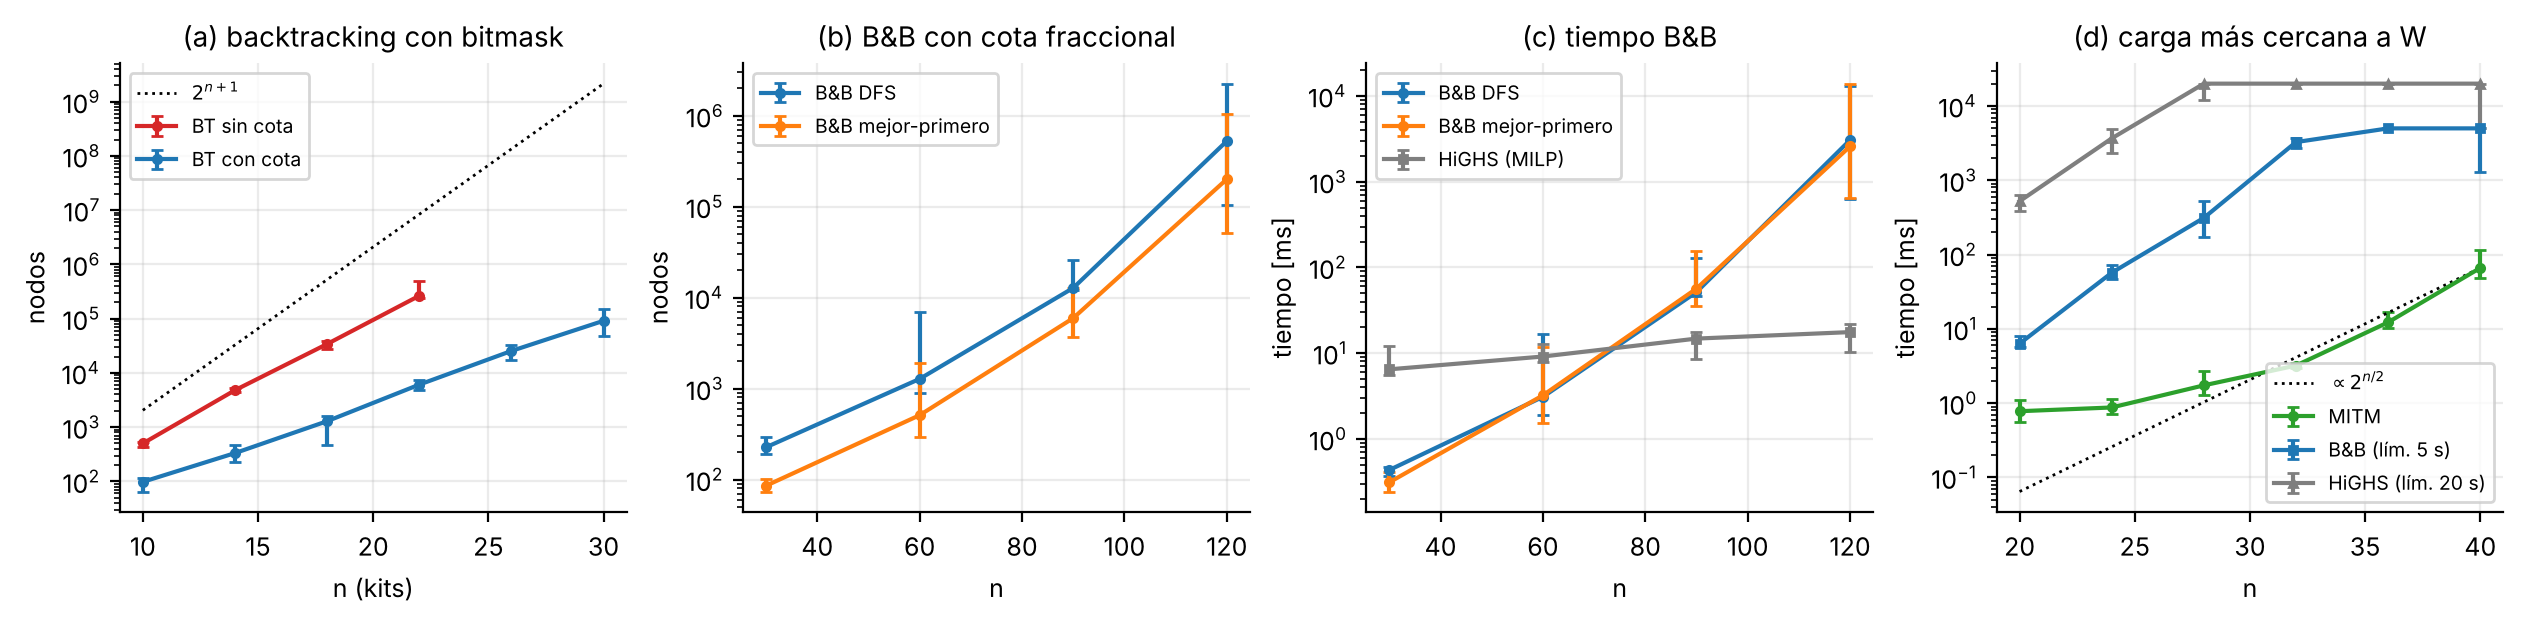
\includegraphics[width=\linewidth]{fig_mochila.png}
\caption{Carga útil (mediana y rango intercuartil de 10 instancias por $n$): (a) backtracking con y
sin cota; (b,c) B\&B con cota fraccional; (d) MITM frente a B\&B y HiGHS para cargar lo más cerca
posible de $W$.}
\label{fig:mochila}
\end{figure}

\begin{table}[t]
\centering\scriptsize
\caption{B\&B con cota fraccional, HiGHS y GA (10 instancias por $n$; GA con 10 semillas por
instancia). ``Termina'': corridas que demostraron optimalidad dentro de 60\,s.}\label{tab:bnb}
\setlength{\tabcolsep}{3pt}
\resizebox{\linewidth}{!}{\begin{tabular}{llrrrrrr}
\toprule
$n$ & método & nodos & tiempo [ms] & mem. [KiB] & brecha [\%] & óptimo [\%] & termina \\
\midrule
\multirow{5}{*}{30} & BT con cota & 86\,115 $\pm$ 87\,883 & 22.12 $\pm$ 21.15 & 9 & 0.000 $\pm$ 0.000 & 100 & -- \\
 & B\&B DFS & 239 $\pm$ 74 & 0.45 $\pm$ 0.11 & 9 & 0.000 $\pm$ 0.000 & 100 & 10/10 \\
 & B\&B mejor-primero & 88 $\pm$ 33 & 0.32 $\pm$ 0.12 & 9 & 0.000 $\pm$ 0.000 & 100 & 10/10 \\
 & HiGHS (MILP) & -- & 30.51 $\pm$ 71.70 & -- & 0.000 $\pm$ 0.000 & 100 & -- \\
 & GA (base bioinspirada) & -- & 75.72 $\pm$ 19.31 & 22 & 0.046 $\pm$ 0.230 & 95 & -- \\
\midrule
\multirow{4}{*}{60} & B\&B DFS & 5\,167 $\pm$ 6\,918 & 12.41 $\pm$ 16.74 & 10 & 0.000 $\pm$ 0.000 & 100 & 10/10 \\
 & B\&B mejor-primero & 1\,887 $\pm$ 2\,708 & 11.59 $\pm$ 17.06 & 21 & 0.000 $\pm$ 0.000 & 100 & 10/10 \\
 & HiGHS (MILP) & -- & 10.37 $\pm$ 3.30 & -- & 0.000 $\pm$ 0.000 & 100 & -- \\
 & GA (base bioinspirada) & -- & 218.12 $\pm$ 28.88 & 28 & 0.387 $\pm$ 0.585 & 51 & -- \\
\midrule
\multirow{4}{*}{90} & B\&B DFS & 26\,466 $\pm$ 33\,395 & 147.72 $\pm$ 242.66 & 11 & 0.000 $\pm$ 0.000 & 100 & 10/10 \\
 & B\&B mejor-primero & 12\,213 $\pm$ 18\,029 & 160.96 $\pm$ 276.09 & 491 & 0.000 $\pm$ 0.000 & 100 & 10/10 \\
 & HiGHS (MILP) & -- & 16.40 $\pm$ 11.40 & -- & 0.000 $\pm$ 0.000 & 100 & -- \\
 & GA (base bioinspirada) & -- & 502.97 $\pm$ 111.63 & 34 & 0.354 $\pm$ 0.736 & 49 & -- \\
\midrule
\multirow{4}{*}{120} & B\&B DFS & 1\,983\,490 $\pm$ 3\,608\,546 & 10\,641.29 $\pm$ 18\,428.13 & 15 & 0.000 $\pm$ 0.000 & 100 & 9/10 \\
 & B\&B mejor-primero & 560\,034 $\pm$ 700\,984 & 7\,783.98 $\pm$ 9\,999.03 & 28\,359 & 0.157 $\pm$ 0.495 & 90 & 9/10 \\
 & HiGHS (MILP) & -- & 21.88 $\pm$ 17.52 & -- & 0.000 $\pm$ 0.000 & 100 & -- \\
 & GA (base bioinspirada) & -- & 740.44 $\pm$ 103.92 & 41 & 0.573 $\pm$ 0.628 & 24 & -- \\
\bottomrule
\end{tabular}
}
\end{table}

\begin{table}[t]
\centering\scriptsize
\caption{MITM para cargar lo más cerca posible de $W$ (10 instancias por $n$).}\label{tab:mitm}
\resizebox{\linewidth}{!}{\begin{tabular}{rrrrrrrrrr}
\toprule
$n$ & MITM [ms] & subconjuntos & $|\partial B|$ & $W-$carga & consistente [\%] & mem. MITM [KiB] & B\&B [ms] & B\&B al límite & mem. B\&B [KiB] \\
\midrule
20 & 1.0 $\pm$ 0.6 & 698 & 2.3 $\pm$ 2.8 & 336.4 & 100 & 79 & 8 $\pm$ 4 & 0/10 & 9 \\
24 & 1.1 $\pm$ 0.6 & 2\,077 & 2.3 $\pm$ 2.6 & 388.0 & 100 & 303 & 73 $\pm$ 57 & 0/10 & 9 \\
28 & 2.2 $\pm$ 1.2 & 7\,584 & 3.2 $\pm$ 2.9 & 463.8 & 100 & 1\,188 & 362 $\pm$ 213 & 0/10 & 9 \\
32 & 3.3 $\pm$ 0.4 & 17\,914 & 0.6 $\pm$ 1.1 & 364.1 & 100 & 4\,740 & 3\,069 $\pm$ 1\,341 & 1/10 & 9 \\
36 & 15.0 $\pm$ 7.0 & 63\,467 & 1.8 $\pm$ 2.9 & 351.3 & 100 & 18\,949 & 4\,503 $\pm$ 1\,575 & 9/10 & 9 \\
40 & 100.5 $\pm$ 91.6 & 260\,230 & 3.4 $\pm$ 3.8 & 320.2 & 100 & 75\,781 & 3\,505 $\pm$ 2\,408 & 7/10 & 10 \\
\bottomrule
\end{tabular}
}
\end{table}

%=====================================================================
\section{Plataformas de aterrizaje y turnos (CSP)}
%=====================================================================

\paragraph{Modelo.} Variables: una por entrega $d$. Dominio:
$D_d=\{(p,t):p\in\text{plataformas permitidas},\ t\in[e_d,l_d]\}$, donde $[e_d,l_d]$ es la
ventana de llegada del dron y los drones pesados sólo pueden usar las plataformas reforzadas
(primera y última fila). Para todo par $d\ne d'$ con valores $(p,t)$ y $(p',t')$:
\[
t\ne t'\ \ \lor\ \ p'\notin N[p],\qquad N[p]=\{p\}\cup\text{vecinos}(p),
\]
es decir, un dron por plataforma por turno y nunca dos plataformas adyacentes a la vez. Los dominios
son \emph{bitsets}: $(p,t)$ es el bit $tP+p$ y $\text{conf}[a]$ es la máscara de los valores
incompatibles con $a$, de modo que forward checking es \texttt{dom[y] \&= \~{}conf[a]}.

\paragraph{Algoritmos.} Backtracking cronológico (BT); forward checking (FC); AC-3, como
preprocesamiento o mantenido en cada nodo (MAC), con \emph{revise}$(X_i,X_j)$: $a$ tiene soporte sii
$D_j\,\&\,\neg\text{conf}[a]\neq0$. En MAC, después de forward checking la cola de AC-3 empieza con los
arcos $(X_k,X_j)$ hacia cada variable $X_j$ cuyo dominio se redujo, para que esas reducciones se
propaguen entre las variables que faltan. MRV elige la variable con menos valores \emph{legales}
restantes (en BT, los del dominio que no chocan con lo ya asignado), con desempate por grado (entregas
con ventana traslapada), y LCV prueba primero el valor que elimina menos valores ajenos. Min-conflicts (10 semillas) sirve de referencia de
búsqueda local. Todas las soluciones se revisaron con un verificador independiente
(\cspValidas\,\% válidas de \cspSoluciones).

\paragraph{Resultados.} Con un hub de $3\times4$ plataformas, adyacencia de 8 y $T=8$ turnos caben
a lo sumo 4 drones por turno (32 en total). La Tabla~\ref{tab:csp} y la Figura~\ref{fig:csp} muestran
la transición de fase: lejos de la capacidad todos resuelven; cerca de ella BT y FC con orden
estático se atoran, MRV es lo que más ayuda y LCV ayuda en las instancias más difíciles. AC-3 sólo
como preprocesamiento no cambia nada: en la raíz todos los valores tienen soporte, porque la restricción
es ``suelta'' (un valor $(p,t)$ pierde soporte en $X_j$ sólo si todo $D_j$ cae en el mismo turno y en la
vecindad de $p$). Mantenido en cada nodo (MAC), en cambio, sí poda más que forward checking cuando los
dominios ya están casi vacíos, que es justo la región difícil: la mediana de nodos baja de \cspNodFcDCI{}
a \cspNodMacDCI{} con $D=28$, de \cspNodFcDDA{} a \cspNodMacDDA{} con $D=30$ y de \cspNodFcDDC{} (el límite) a
\cspNodMacDDC{} con $D=32$, comparado con FC+MRV+LCV. Cada nodo de MAC cuesta mucho más, porque AC-3
revisa hasta $O(D^2)$ arcos (\cspTMacDDA\,ms contra \cspTFcDDA\,ms en promedio con $D=30$), así que con el
límite de 5\,s las dos variantes terminan proporciones parecidas de instancias (\cspDoneMacDDA{} y
\cspDoneFcDDA{} con $D=30$). Ninguno de los métodos completos prueba rápido la insatisfacibilidad de las
instancias saturadas (son problemas tipo palomar), y min-conflicts nunca puede probarla.

\begin{table}[t]
\centering\scriptsize
\caption{CSP con hub de $3\times4$ y $T=8$ (10 instancias por $D$). Por método: \% de instancias
terminadas dentro de $10^5$ nodos o 5\,s (mediana de nodos); min-conflicts: \% resueltas.}
\label{tab:csp}
\resizebox{\linewidth}{!}{\begin{tabular}{rrrrrrrrrr}
\toprule
$D$ & \makecell{sat/unsat\\/?} & BT & BT+MRV & FC & FC+MRV & \makecell{FC+MRV\\+LCV} & \makecell{AC-3+FC\\+MRV+LCV} & \makecell{MAC+MRV\\+LCV} & \makecell{Min-\\conflicts} \\
\midrule
12 & 10/0/0 & 100 (35) & 100 (36) & 100 (12) & 100 (12) & 100 (12) & 100 (12) & 100 (12) & 100 \\
16 & 10/0/0 & 90 (55) & 100 (53) & 100 (16) & 100 (16) & 100 (16) & 100 (16) & 100 (16) & 100 \\
20 & 10/0/0 & 80 (102) & 100 (93) & 90 (21) & 100 (20) & 100 (20) & 100 (20) & 100 (20) & 100 \\
22 & 10/0/0 & 80 (96) & 100 (98) & 80 (22) & 100 (22) & 100 (22) & 100 (22) & 100 (22) & 100 \\
24 & 10/0/0 & 40 (100\,002) & 100 (157) & 80 (33) & 100 (24) & 100 (24) & 100 (24) & 100 (24) & 100 \\
26 & 9/0/1 & 30 (100\,000) & 80 (186) & 40 (100\,000) & 90 (26) & 90 (26) & 90 (26) & 90 (26) & 90 \\
28 & 3/3/4 & 0 (100\,009) & 50 (52\,583) & 0 (100\,000) & 50 (50\,216) & 60 (422) & 60 (422) & 60 (196) & 30 \\
30 & 6/1/3 & 0 (100\,010) & 20 (100\,009) & 10 (100\,000) & 30 (100\,000) & 60 (16\,243) & 60 (16\,243) & 50 (3\,599) & 67 \\
32 & 1/1/8 & 0 (100\,006) & 10 (100\,012) & 0 (100\,000) & 10 (100\,000) & 20 (100\,000) & 20 (100\,000) & 20 (24\,192) & 18 \\
\bottomrule
\end{tabular}
}
\end{table}

\begin{figure}[t]
\centering
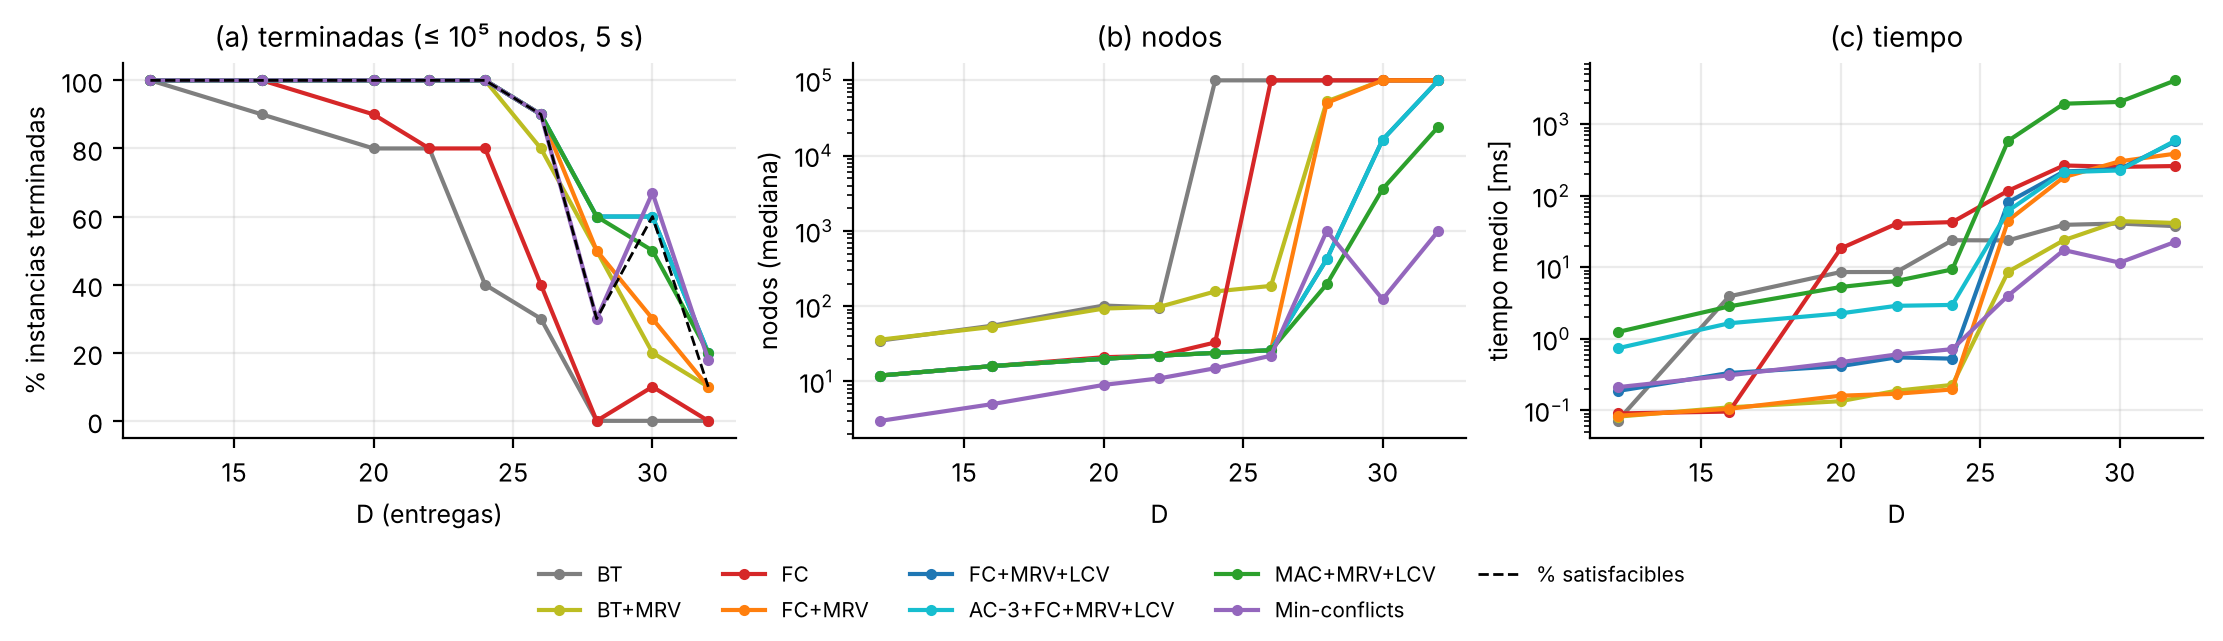
\includegraphics[width=\linewidth]{fig_csp.png}
\caption{Transición de fase del CSP de plataformas y turnos.}
\label{fig:csp}
\end{figure}

\begin{table}[H]
\centering\scriptsize
\caption{Escalamiento con un hub de $4\times5$, adyacencia de 4 y $T=12$: \% terminadas / tiempo
medio [ms].}\label{tab:cspesc}
\begin{tabular}{rrrrrr}
\toprule
$D$ & BT+MRV & FC+MRV & FC+MRV+LCV & MAC+MRV+LCV & Min-conflicts \\
\midrule
20 & 100 / 0.3 & 100 / 0.3 & 100 / 1.3 & 100 / 13.0 & 100 / 0.5 \\
40 & 100 / 0.5 & 100 / 0.6 & 100 / 2.9 & 100 / 62.7 & 100 / 1.0 \\
60 & 100 / 0.9 & 100 / 1.0 & 100 / 6.3 & 100 / 210.1 & 100 / 2.2 \\
80 & 100 / 1.4 & 100 / 1.8 & 100 / 9.2 & 100 / 452.9 & 100 / 3.7 \\
100 & 80 / 10.2 & 80 / 163.3 & 100 / 12.0 & 100 / 858.9 & 100 / 21.1 \\
\bottomrule
\end{tabular}

\end{table}

{\sloppy En el hub grande todas las instancias resultaron satisfacibles y FC+MRV+LCV y MAC+MRV+LCV las
resuelven sin retroceder (exactamente $D$ nodos), así que la propagación extra de MAC no tiene nada que
ahorrar y sólo cuesta: con $D=\cspDmax$, FC+MRV+LCV tardó \cspTFc\,ms y MAC+MRV+LCV \cspTMac\,ms en
promedio, con memoria pico de \cspMemFc{} y \cspMemMac\,KiB (Tabla~\ref{tab:cspmem}). Con bitsets, guardar
una copia de los dominios por nivel es barato; lo que ocupa memoria en MAC es la cola de AC-3. BT+MRV
usa la menor memoria (\cspMemBt\,KiB) porque no copia dominios, pero con $D=\cspDmax$ ya no terminó todas
las instancias. Min-conflicts resolvió todas usando \cspMemMc\,KiB.\par}

\begin{table}[H]
\centering\scriptsize
\caption{Memoria pico de Python [KiB] en el hub de $4\times5$ (instancia 0 de cada $D$; min-conflicts con
la semilla 0).}\label{tab:cspmem}
\begin{tabular}{lrrrrr}
\toprule
método & $D=20$ & $D=40$ & $D=60$ & $D=80$ & $D=100$ \\
\midrule
BT+MRV & 18 & 28 & 43 & 62 & 72 \\
FC+MRV & 24 & 51 & 94 & 149 & 212 \\
FC+MRV+LCV & 24 & 50 & 93 & 150 & 211 \\
MAC+MRV+LCV & 45 & 175 & 275 & 930 & 1\,155 \\
Min-conflicts & 46 & 54 & 66 & 76 & 84 \\
\bottomrule
\end{tabular}

\end{table}

%=====================================================================
\section{Orden de visita: TSP asimétrico}
%=====================================================================

La matriz $C\in\mathbb R^{(K+1)\times(K+1)}$ se obtiene con Dijkstra dirigido desde el depósito y
cada clínica; por el viento $C\ne C^\top$. Un recorrido es una permutación de las clínicas que sale y
regresa al depósito.

\subsection{Métodos exactos}
\begin{prop}
Para un prefijo $0\to\dots\to u$ con costo $g$ y conjunto restante $R$, con
$s_{ij}=\min(c_{ij},c_{ji})$,
\[
LB=\max\Bigl\{g+\mathrm{MST}_s(R\cup\{u,0\}),\ \ g+\mathrm{MST}_s(R)+\min_{r\in R}c_{ur}+\min_{r\in R}c_{r0}\Bigr\}
\]
es una cota inferior del costo de cualquier recorrido que extienda el prefijo.
\end{prop}
\begin{proof}
El resto del recorrido es un camino hamiltoniano $u\to R\to0$. Ignorando direcciones es un árbol de
expansión de $R\cup\{u,0\}$, y cada arista dirigida cuesta al menos su $s_{ij}$; eso da la primera
cota. Quitando las dos aristas extremas queda un camino que es árbol de expansión de $R$, y esas dos
aristas cuestan al menos $\min_r c_{ur}$ y $\min_r c_{r0}$.
\end{proof}
El B\&B es en profundidad, ordena los hijos por $c_{ur}$ y poda con $LB\ge$ mejor. Se comparó sin
cota inicial, con la cota del vecino más cercano (VMC) y con la de ACO+LS (híbrido exacto +
bioinspirado). Held--Karp ($O(2^KK^2)$) y la fuerza bruta ($K\le8$) sirven de control. Para
$K>12$ el óptimo se obtuvo con HiGHS: formulación de asignación con cortes de 2-ciclos y cortes de
subciclos de Dantzig--Fulkerson--Johnson agregados de forma perezosa (a lo sumo \milpMaxT\,s por
instancia). Como HiGHS declara óptimo dentro de una tolerancia relativa ($10^{-4}$ por omisión), las 16
instancias se resolvieron otra vez con tolerancia 0 y los óptimos fueron idénticos; además, ninguna de
las 1\,120 corridas de metaheurísticas encontró un recorrido más barato. La relajación de asignación
(AP) queda en promedio \apGap\,\% por debajo del óptimo.

\begin{table}[t]
\centering\scriptsize
\caption{ATSP exacto con $K\le12$ ($N=100$, 10 subconjuntos de clínicas por $K$). Para Held--Karp
se reportan los estados $2^KK$; el tiempo de ``+ACO+LS'' incluye 2\,000 evaluaciones de ACO+LS.}
\label{tab:atspex}
\begin{tabular}{llrrrr}
\toprule
$K$ & método & nodos / estados & tiempo [ms] & mem. [KiB] & óptimo [\%] \\
\midrule
\multirow{5}{*}{6} & Fuerza bruta & 720 $\pm$ 0 & 3.8 $\pm$ 1.9 & 3.8 & 100 \\
 & Held--Karp (DP) & 384 $\pm$ 0 & 1.4 $\pm$ 0.6 & 10.8 & 100 \\
 & B\&B (MST) & 87 $\pm$ 45 & 1.3 $\pm$ 0.6 & 7.5 & 100 \\
 & B\&B (MST) + VMC & 85 $\pm$ 45 & 1.3 $\pm$ 0.7 & 7.5 & 100 \\
 & B\&B (MST) + ACO+LS & 76 $\pm$ 44 & 40.4 $\pm$ 17.4 & 7.3 & 100 \\
\midrule
\multirow{5}{*}{8} & Fuerza bruta & 40\,320 $\pm$ 0 & 168.3 $\pm$ 31.7 & 3.9 & 100 \\
 & Held--Karp (DP) & 2\,048 $\pm$ 0 & 5.6 $\pm$ 1.4 & 38.3 & 100 \\
 & B\&B (MST) & 422 $\pm$ 543 & 8.8 $\pm$ 8.2 & 10.4 & 100 \\
 & B\&B (MST) + VMC & 419 $\pm$ 543 & 8.8 $\pm$ 8.4 & 10.4 & 100 \\
 & B\&B (MST) + ACO+LS & 394 $\pm$ 546 & 43.6 $\pm$ 12.8 & 10.2 & 100 \\
\midrule
\multirow{4}{*}{10} & Held--Karp (DP) & 10\,240 $\pm$ 0 & 29.1 $\pm$ 6.9 & 207.9 & 100 \\
 & B\&B (MST) & 2\,463 $\pm$ 2\,930 & 113.9 $\pm$ 117.4 & 14.0 & 100 \\
 & B\&B (MST) + VMC & 2\,461 $\pm$ 2\,929 & 97.7 $\pm$ 88.7 & 14.0 & 100 \\
 & B\&B (MST) + ACO+LS & 2\,383 $\pm$ 2\,938 & 132.6 $\pm$ 93.7 & 13.9 & 100 \\
\midrule
\multirow{4}{*}{12} & Held--Karp (DP) & 49\,152 $\pm$ 0 & 148.8 $\pm$ 31.2 & 983.6 & 100 \\
 & B\&B (MST) & 22\,702 $\pm$ 36\,744 & 1\,077.8 $\pm$ 1\,416.6 & 18.2 & 100 \\
 & B\&B (MST) + VMC & 22\,700 $\pm$ 36\,744 & 1\,031.1 $\pm$ 1\,391.0 & 18.1 & 100 \\
 & B\&B (MST) + ACO+LS & 20\,504 $\pm$ 31\,160 & 992.4 $\pm$ 1\,238.9 & 17.9 & 100 \\
\bottomrule
\end{tabular}

\end{table}

Con $K=12$ el B\&B con cota MST expandió \exBbNodos{} nodos en promedio (\exBbT\,ms, \exBbMem\,KiB de memoria
pico, frente a \exHkMem\,KiB de la tabla de Held--Karp); con la cota
inicial de ACO+LS bajó a \exBbAcoNodos{} (\exBbAcoT\,ms incluyendo ACO), y con la del vecino más
cercano casi no cambió. Held--Karp tardó \exHkT\,ms. Todos los métodos exactos coincidieron
(\exTodosOk\,\%). Con este tamaño la DP gana: $2^KK^2$ es pequeño, mientras que la cota MST pierde fuerza
con la asimetría (usa $\min(c_{ij},c_{ji})$ e ignora la dirección). La cota inicial ayuda poco porque el
B\&B, al visitar primero los hijos más baratos, encuentra pronto incumbentes casi óptimas; lo que
domina es demostrar que no hay nada mejor.

\begin{figure}[t]
\centering
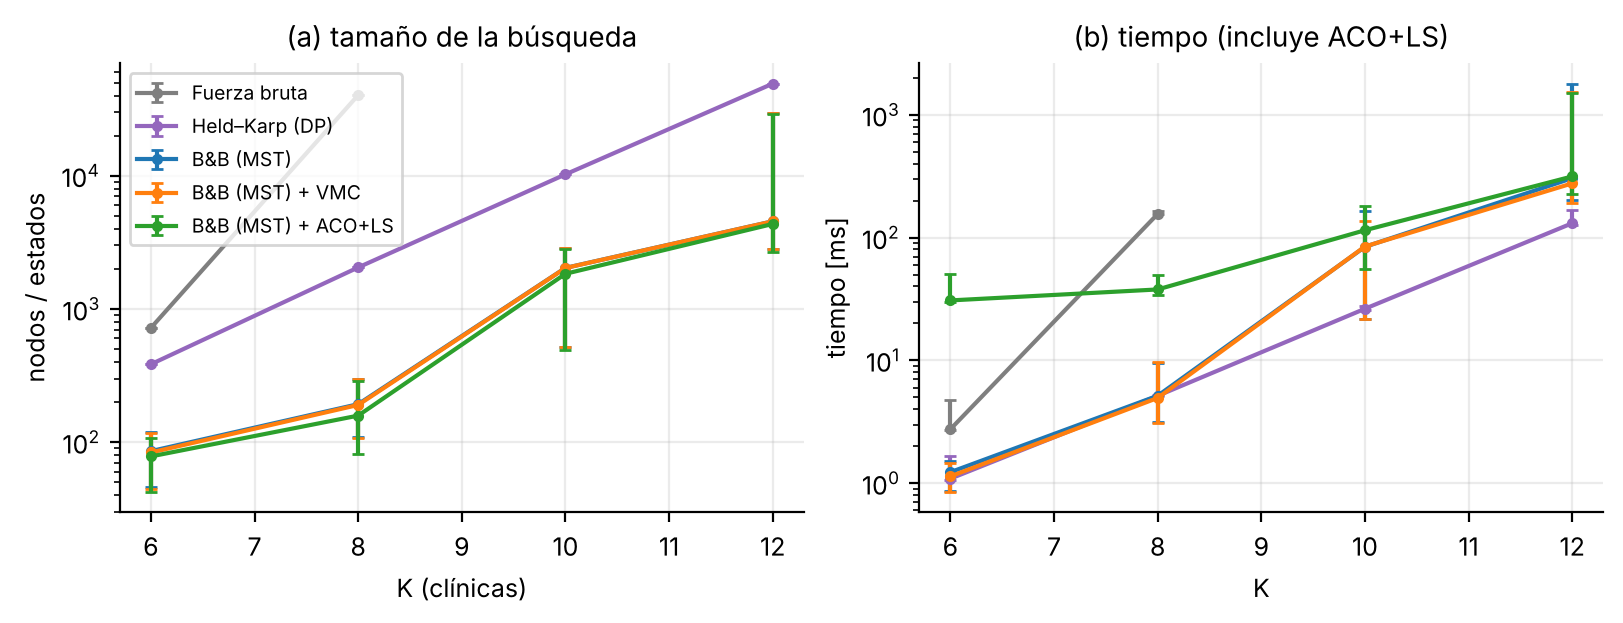
\includegraphics[width=0.85\linewidth]{fig_atsp_exacto.png}
\caption{ATSP exacto con $K\le12$: nodos (estados para Held--Karp, permutaciones para fuerza bruta) y
tiempo; mediana y rango intercuartil de 10 instancias por $K$.}
\label{fig:atspex}
\end{figure}

\subsection{Metaheurísticas}
Todas empiezan de permutaciones aleatorias y tienen el mismo presupuesto de $3\cdot10^4$
evaluaciones de la función objetivo (cada recorrido construido o vecino evaluado cuenta una vez).
\begin{itemize}
\item \textbf{SA}: vecino aleatorio entre swap, inserción y 2-opt (que en el ATSP invierte el sentido
del segmento); $T_0$ calibrada para aceptar la mitad de los empeoramientos y enfriamiento geométrico
hasta $10^{-3}T_0$.
\item \textbf{Tabú}: lista de candidatos de 30 vecinos por iteración (70\,\% inserciones granulares
de una ciudad junto a uno de sus 10 predecesores más baratos, como en la búsqueda tabú granular de
Toth y Vigo, y 30\,\% swap/2-opt); atributo tabú: las ciudades movidas, con permanencia $\approx K/4$;
aspiración por mejora global.
\item \textbf{GA-OX}: población 60, torneo de 3, cruza OX (Davis), mutación por inversión
($p=0.5$) y elitismo de 2.
\item \textbf{ACO (MMAS)}: 20 hormigas, $\alpha=1$, $\beta=3$, $\rho=0.1$, límites
$\tau_{\min},\tau_{\max}$ de Stützle y Hoos; depósito alternado entre la mejor de la iteración y la
global; construcción vectorizada.
\item \textbf{UCB-HH}: hiperheurística de selección; UCB1 elige el operador (swap, inserción o
2-opt) con recompensa 1 si mejora la solución actual; aceptación de SA con la misma temperatura.
\item \textbf{Híbridos} (puntos extra): GA memético (población 30 y búsqueda local granular de $2K$
evaluaciones en el 2\,\% de los hijos) y ACO+LS (búsqueda local sobre la mejor hormiga de cada
iteración); además el B\&B con cota inicial de ACO+LS de la sección anterior.
\end{itemize}

\begin{table}[t]
\centering\scriptsize
\caption{Brecha contra el óptimo exacto [\%] (media $\pm$ d.e. de 10 semillas) para las 16
combinaciones $(N,K)$. En negritas el mejor promedio de cada fila.}
\label{tab:atspmeta}
\setlength{\tabcolsep}{3pt}
\resizebox{\linewidth}{!}{\begin{tabular}{rrrrrrrrrr}
\toprule
$K$ & $N$ & óptimo & SA & Tabu & GA-OX & ACO (MMAS) & UCB-HH & GA memético & ACO+LS \\
\midrule
12 & 50 & 132.0 & \textbf{0.00 $\pm$ 0.00} & \textbf{0.00 $\pm$ 0.00} & \textbf{0.00 $\pm$ 0.00} & \textbf{0.00 $\pm$ 0.00} & \textbf{0.00 $\pm$ 0.00} & \textbf{0.00 $\pm$ 0.00} & \textbf{0.00 $\pm$ 0.00} \\
12 & 100 & 289.5 & \textbf{0.00 $\pm$ 0.00} & \textbf{0.00 $\pm$ 0.00} & \textbf{0.00 $\pm$ 0.00} & \textbf{0.00 $\pm$ 0.00} & \textbf{0.00 $\pm$ 0.00} & \textbf{0.00 $\pm$ 0.00} & \textbf{0.00 $\pm$ 0.00} \\
12 & 150 & 491.3 & \textbf{0.00 $\pm$ 0.00} & \textbf{0.00 $\pm$ 0.00} & \textbf{0.00 $\pm$ 0.00} & \textbf{0.00 $\pm$ 0.00} & \textbf{0.00 $\pm$ 0.00} & \textbf{0.00 $\pm$ 0.00} & \textbf{0.00 $\pm$ 0.00} \\
12 & 200 & 648.8 & \textbf{0.00 $\pm$ 0.00} & \textbf{0.00 $\pm$ 0.00} & 0.16 $\pm$ 0.35 & 0.33 $\pm$ 0.43 & \textbf{0.00 $\pm$ 0.00} & 0.16 $\pm$ 0.35 & 0.41 $\pm$ 0.43 \\
25 & 50 & 206.8 & \textbf{0.00 $\pm$ 0.00} & 0.45 $\pm$ 0.95 & 1.69 $\pm$ 1.59 & \textbf{0.00 $\pm$ 0.00} & 0.45 $\pm$ 0.95 & 0.84 $\pm$ 1.43 & \textbf{0.00 $\pm$ 0.00} \\
25 & 100 & 369.7 & 0.26 $\pm$ 0.83 & 0.33 $\pm$ 0.93 & 2.23 $\pm$ 1.21 & 1.84 $\pm$ 0.00 & \textbf{0.00 $\pm$ 0.00} & 0.59 $\pm$ 1.24 & \textbf{0.00 $\pm$ 0.00} \\
25 & 150 & 642.1 & \textbf{0.00 $\pm$ 0.00} & \textbf{0.00 $\pm$ 0.00} & 1.82 $\pm$ 1.70 & 1.29 $\pm$ 0.88 & \textbf{0.00 $\pm$ 0.00} & 1.04 $\pm$ 1.67 & \textbf{0.00 $\pm$ 0.00} \\
25 & 200 & 874.7 & 0.39 $\pm$ 0.82 & \textbf{0.00 $\pm$ 0.00} & \textbf{0.00 $\pm$ 0.00} & 1.09 $\pm$ 0.80 & \textbf{0.00 $\pm$ 0.00} & 0.32 $\pm$ 1.01 & 0.27 $\pm$ 0.56 \\
50 & 50 & 251.9 & 5.62 $\pm$ 2.60 & 3.91 $\pm$ 3.06 & 8.03 $\pm$ 2.97 & 2.65 $\pm$ 1.38 & 2.56 $\pm$ 2.41 & 5.60 $\pm$ 3.09 & \textbf{1.99 $\pm$ 1.28} \\
50 & 100 & 475.9 & 4.64 $\pm$ 1.60 & 3.73 $\pm$ 2.16 & 10.84 $\pm$ 4.17 & 6.28 $\pm$ 1.07 & 4.63 $\pm$ 2.57 & 4.53 $\pm$ 1.11 & \textbf{3.61 $\pm$ 1.29} \\
50 & 150 & 799.1 & 3.23 $\pm$ 4.28 & 4.65 $\pm$ 4.07 & 11.49 $\pm$ 4.38 & 3.64 $\pm$ 1.39 & 1.62 $\pm$ 2.61 & 3.39 $\pm$ 3.89 & \textbf{0.94 $\pm$ 1.19} \\
50 & 200 & 1\,107.7 & \textbf{1.75 $\pm$ 1.65} & 3.49 $\pm$ 3.90 & 8.44 $\pm$ 5.01 & 3.17 $\pm$ 1.58 & 1.81 $\pm$ 1.25 & 3.88 $\pm$ 2.90 & 2.33 $\pm$ 1.32 \\
100 & 50 & 331.2 & 11.42 $\pm$ 2.99 & 12.20 $\pm$ 5.41 & 83.71 $\pm$ 11.44 & 9.37 $\pm$ 1.49 & 10.04 $\pm$ 2.21 & 22.90 $\pm$ 4.42 & \textbf{8.91 $\pm$ 1.81} \\
100 & 100 & 693.6 & 12.62 $\pm$ 3.60 & 9.36 $\pm$ 3.29 & 85.23 $\pm$ 11.56 & 10.23 $\pm$ 1.63 & 10.18 $\pm$ 2.69 & 24.04 $\pm$ 5.46 & \textbf{6.93 $\pm$ 1.34} \\
100 & 150 & 1\,117.1 & 14.02 $\pm$ 2.90 & 11.69 $\pm$ 4.80 & 85.46 $\pm$ 11.89 & 9.25 $\pm$ 1.83 & 11.69 $\pm$ 3.26 & 23.43 $\pm$ 7.14 & \textbf{8.91 $\pm$ 2.71} \\
100 & 200 & 1\,447.0 & 12.84 $\pm$ 4.88 & 14.11 $\pm$ 5.54 & 86.92 $\pm$ 15.17 & 9.17 $\pm$ 2.07 & \textbf{8.86 $\pm$ 4.06} & 26.18 $\pm$ 9.85 & 9.71 $\pm$ 2.42 \\
\bottomrule
\end{tabular}
}
\end{table}

\begin{figure}[t]
\centering
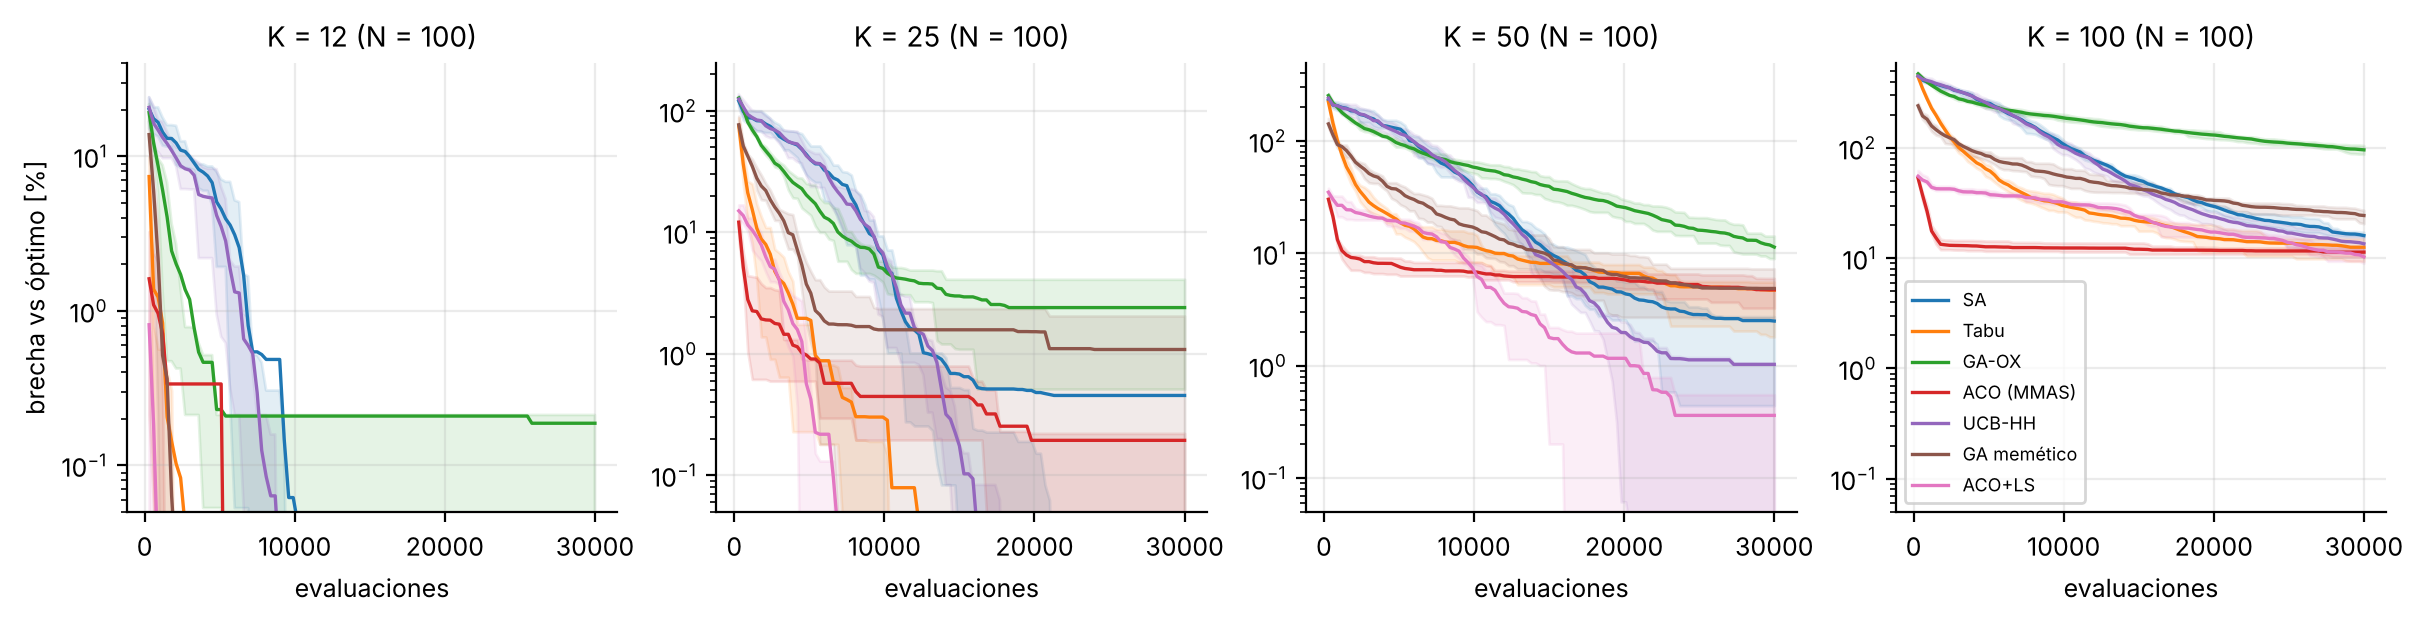
\includegraphics[width=\linewidth]{fig_atsp_convergencia.png}
\caption{Convergencia con $N=100$: brecha contra el óptimo (línea: media de 10 semillas; banda: rango
intercuartil). Las brechas nulas se dibujan en $10^{-3}$ por la escala logarítmica.}
\label{fig:conv}
\end{figure}

\begin{figure}[t]
\centering
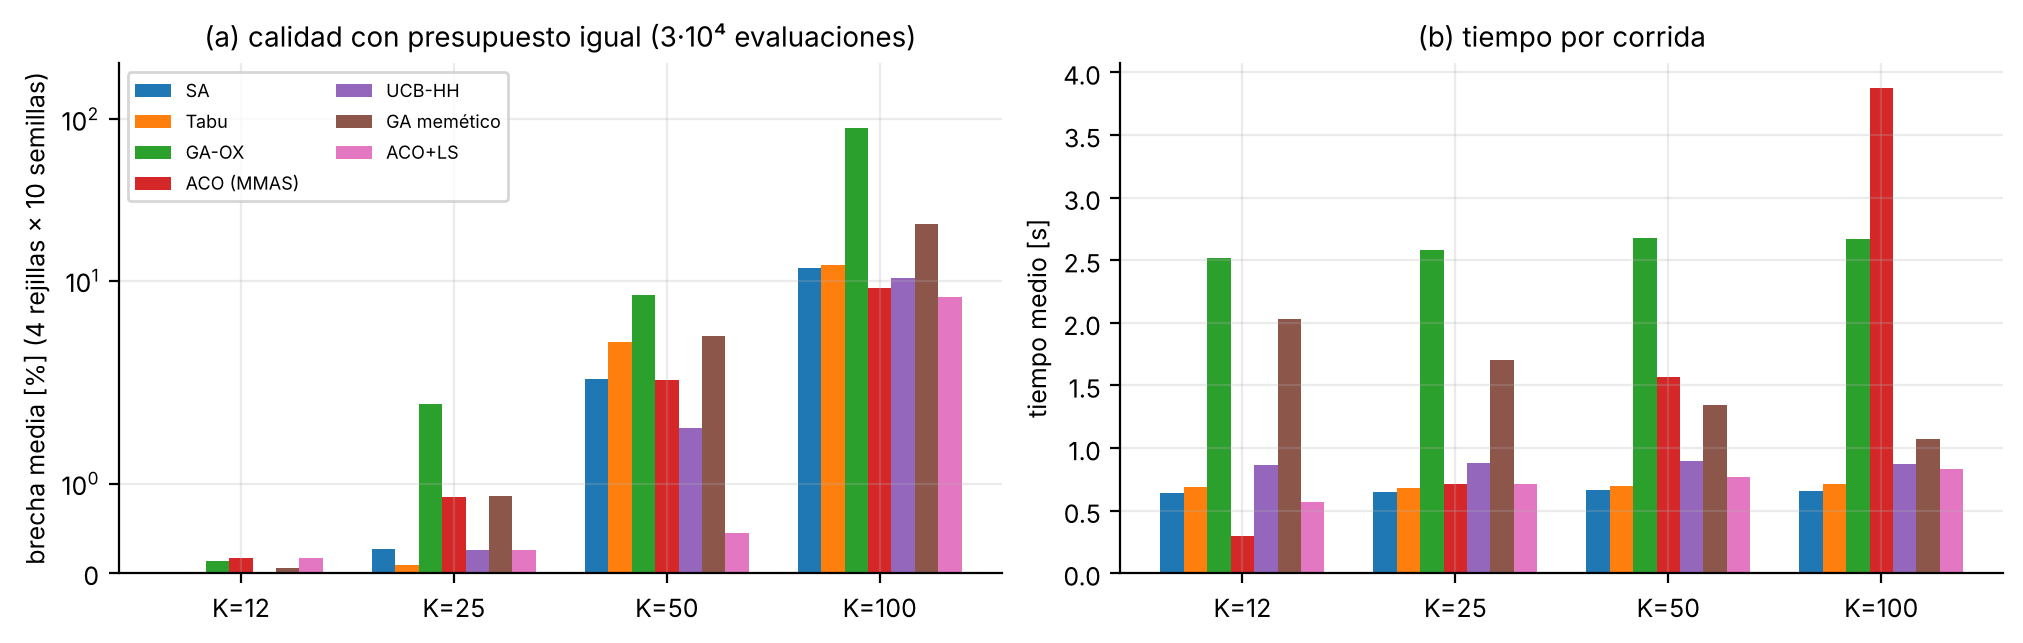
\includegraphics[width=\linewidth]{fig_atsp_brechas.png}
\caption{Brecha media y tiempo por corrida, promediados sobre las cuatro rejillas.}
\label{fig:brechas}
\end{figure}

\begin{table}[H]
\centering\scriptsize
\caption{Tiempo medio por corrida [s] / memoria pico de Python [KiB]. La memoria se midió con la
semilla 0 y $5\,000$ evaluaciones: el pico lo fijan la población o la matriz de feromona, no el
número de evaluaciones.}
\label{tab:atsptiempo}
\setlength{\tabcolsep}{3pt}
\begin{tabular}{rrrrrrrr}
\toprule
$K$ & SA & Tabu & GA-OX & ACO (MMAS) & UCB-HH & GA memético & ACO+LS \\
\midrule
12 & 0.64 / 12 & 0.69 / 14 & 2.52 / 41 & 0.30 / 37 & 0.86 / 31 & 2.03 / 32 & 0.57 / 37 \\
25 & 0.65 / 16 & 0.68 / 23 & 2.58 / 59 & 0.71 / 68 & 0.88 / 31 & 1.71 / 43 & 0.71 / 72 \\
50 & 0.67 / 18 & 0.70 / 49 & 2.68 / 101 & 1.57 / 186 & 0.89 / 34 & 1.34 / 75 & 0.77 / 205 \\
100 & 0.66 / 21 & 0.71 / 169 & 2.67 / 195 & 3.88 / 613 & 0.87 / 36 & 1.07 / 181 & 0.83 / 691 \\
\bottomrule
\end{tabular}

\end{table}

\paragraph{Resultados.} Con $K=12$ todos los métodos quedan a menos de 0.2\,\% del óptimo, y SA, Tabú y
UCB-HH lo encuentran en las 40 corridas. La diferencia aparece al crecer $K$: el mejor promedio fue
\mejorKCF{} con $K=25$ (\mejorGapKCF\,\%), \mejorKFA{} con $K=50$ (\mejorGapKFA\,\%) y \mejorKBAA{}
con $K=100$ (\mejorGapKBAA\,\%). Con $K=100$ las brechas medias fueron: SA \gapSaKBAA, Tabú
\gapTabuKBAA, GA-OX \gapGaKBAA, ACO \gapAcoKBAA, UCB-HH \gapUcbKBAA, memético \gapMemKBAA{} y ACO+LS
\gapAcoLsKBAA\,\%. Algunas conclusiones:
\begin{itemize}
\item El GA puro es el más débil con presupuesto fijo: OX conserva el orden relativo, pero recombinar
sin búsqueda local avanza muy despacio en un espacio de $K!$ permutaciones. Agregarle búsqueda local
(memético) reduce su brecha a la cuarta parte con $K=100$.
\item ACO+LS fue el más robusto para $K\ge50$: la feromona concentra la construcción en aristas
buenas y la búsqueda local granular corrige el detalle. ACO sin búsqueda local también escala bien
en calidad, pero es el más lento con $K=100$ porque cada construcción cuesta $O(K^2)$.
\item UCB-HH superó a SA, que usa la misma aceptación y temperatura pero elige el operador al azar,
en $K=50$ y $K=100$. En promedio UCB eligió 2-opt el \ucbTwo\,\%, inserción el \ucbIns\,\% y swap el
\ucbSwap\,\% de las veces (Figura~\ref{fig:ucb}): aprendió que invertir segmentos mejora más seguido.
\item El tamaño de la rejilla $N$ no muestra una tendencia clara: sólo cambia la matriz $C$, y la
brecha depende sobre todo de $K$.
\item Con $K=100$ las curvas de la Figura~\ref{fig:conv} siguen bajando al final del presupuesto: con
más evaluaciones todos mejorarían, y el orden entre métodos se mantiene a lo largo de la curva.
\end{itemize}

\begin{figure}[H]
\centering
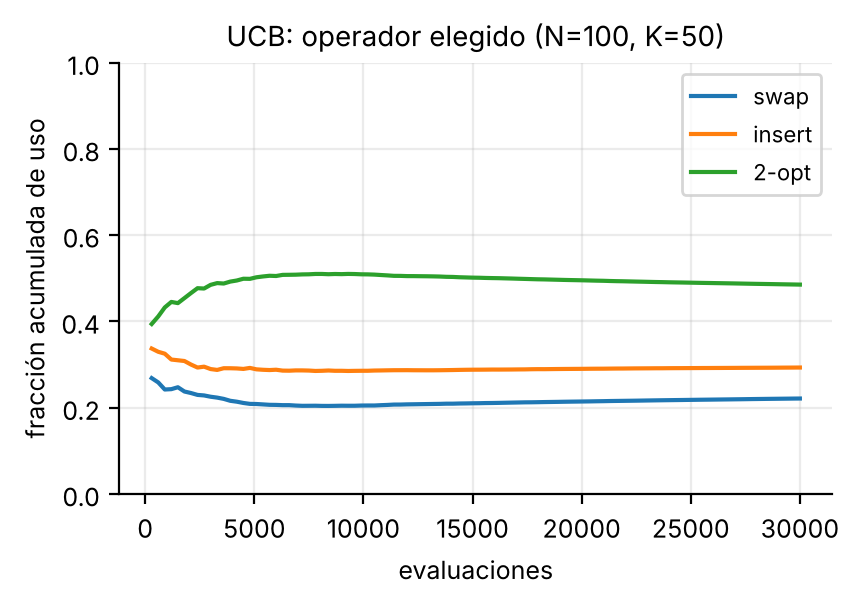
\includegraphics[width=0.5\linewidth]{fig_ucb.png}
\caption{Fracción acumulada de uso de cada operador en la hiperheurística UCB ($N=100$, $K=50$,
media de 10 semillas).}
\label{fig:ucb}
\end{figure}

%=====================================================================
\section{Discusión: qué garantiza cada método}
%=====================================================================

\begin{table}[H]
\centering\small
\caption{Garantías de los métodos usados.}\label{tab:garantias}
\begin{tabular}{p{4.2cm}p{11.3cm}}
\toprule
Método & Garantía \\
\midrule
UCS, A* ($h$ consistente), IDA*/IDA*-CR & \textbf{Exactos}: completos y óptimos (costos $>0$). A* no
reabre nodos y es óptimamente eficiente para su $h$; IDA* usa $O(d)$ memoria sin TT. \\
A* ponderado ($w$) & Completo, costo $\le w\,C^*$ demostrable. \\
A* con $h_\theta$ aprendida & Completo (grafo finito, con reapertura). Pierde la optimalidad, la
consistencia (hay reaperturas) y la cota a priori: $C\le w_PC^*$ sólo vale para el $w_P$
\emph{medido}, que no se conoce antes de resolver y puede crecer fuera de la distribución de
entrenamiento. \\
Backtracking, B\&B, MITM, Held--Karp, B\&B-MST, HiGHS & \textbf{Exactos}. \\
BT, FC, MAC (CSP) & \textbf{Completos}: deciden satisfacible/insatisfacible (si terminan). \\
Min-conflicts & Incompleto: no puede demostrar insatisfacibilidad. \\
SA & \textbf{Probabilísticamente completo} sólo con enfriamiento logarítmico (Hajek, 1988); con el
enfriamiento geométrico usado no hay garantía. \\
GA elitista con mutación & Converge en probabilidad al óptimo (Rudolph, 1994): la inversión genera
cualquier permutación con probabilidad positiva y el elitismo no pierde lo encontrado. \\
ACO (MMAS) & $\tau_{\min}>0$ da convergencia en valor: la probabilidad de haber construido el óptimo
tiende a 1 (Stützle y Dorigo, 2002). \\
Tabú, UCB-HH & Sin garantía de optimalidad. La cota de regret de UCB1 supone recompensas
estacionarias, y aquí la utilidad de cada operador cambia durante la búsqueda. \\
\bottomrule
\end{tabular}
\end{table}

\paragraph{Memoria.} Las diferencias de memoria siguen a las estructuras de datos. A* y UCS guardan
$g$, padres y frontera para toda la rejilla ($O(V)$; con $N=200$, \memAstarNCAA{} y \memUcsNCAA\,KiB en
promedio). IDA* sin tabla de transposición sólo guarda la pila ($O(d)$), pero en rejillas eso lo
vuelve impráctico; con la tabla vuelve a $O(V)$ (\memIdaCrNCAA\,KiB para IDA*-CR con $N=200$). En la
mochila, la DFS guarda una rama ($O(n)$) y mejor-primero toda la frontera (hasta \bnbBestMemMax\,MiB),
y MITM sus $2^{n/2}$ subconjuntos por mitad (\mitmMem\,MiB con $n=40$). Held--Karp necesita su tabla de
$2^K K$ estados, MAC una cola de hasta $O(D^2)$ arcos, ACO la matriz de feromona $O(K^2)$
(\memMetaAco\,KiB con $K=100$) y SA, Tabú y UCB-HH sólo un par de permutaciones (\memMetaSa{} y
\memMetaTabu\,KiB).

En resumen, para las decisiones que sí admiten demostración en el tiempo disponible conviene usar
los métodos exactos con buenas cotas: A* con la heurística consistente para las rutas (milisegundos en
rejillas de $200\times200$), B\&B con cota fraccional para la carga (casi siempre en milisegundos con
$n\le120$, aunque con instancias difíciles cuando los kits densos son incompatibles) y Held--Karp para
$K\le12$. Cuando el problema crece, las metaheurísticas híbridas dan buenas soluciones en menos de un
segundo (ACO+LS: \mejorGapKFA\,\% con $K=50$ y \mejorGapKBAA\,\% con $K=100$), pero sólo un método
exacto (aquí HiGHS con cortes, hasta \milpMaxT\,s) puede certificar la brecha. La heurística aprendida
muestra el intercambio central: renuncia a las garantías a cambio de información; en la escala de
entrenamiento ahorra nodos, fuera de ella deja de ayudar, y A* ponderado da un ahorro parecido con una
cota demostrable.

%=====================================================================
\section{Puntos extra}
%=====================================================================
\begin{itemize}
\item \textbf{Panel interactivo} (\texttt{dashboard/panel\_drones.html}, un solo archivo sin
dependencias): mapa de la misión con capas de viento, rutas de cada método y nodos expandidos;
curvas de convergencia para las 16 combinaciones $(N,K)$; tablas de búsqueda, mochila y CSP; y el
horario de plataformas.
\item \textbf{Heurística aprendida} con dos pérdidas, verificación empírica de la
Proposición~\ref{prop:w} y su prueba.
\item \textbf{Híbridos búsqueda--bioinspirados}: GA memético, ACO+LS y B\&B exacto con cota inicial
de ACO+LS.
\end{itemize}

%=====================================================================
\section{Configuración experimental y reproducibilidad}
%=====================================================================
\begin{itemize}
\item \textbf{Hardware}: Intel Xeon @ 2.10\,GHz, 2 vCPU, 7\,GB de RAM, Linux. Python 3.13.18,
NumPy 2.5.3, SciPy 1.18.1 (Dijkstra, HiGHS), scikit-learn 1.9.1.
\item \textbf{Tiempo}: \texttt{time.perf\_counter}, sin instrumentar. \textbf{Memoria}: pico de
asignaciones de Python con \texttt{tracemalloc} en una corrida aparte (no incluye el intérprete).
\item \textbf{Semillas}: los métodos estocásticos (SA, Tabú, GA, ACO, UCB-HH, híbridos, GA de la
mochila, min-conflicts) se corrieron con 10 semillas. Las tablas reportan media $\pm$ desviación
estándar; las figuras con escala logarítmica, mediana y rango intercuartil. Los métodos deterministas
se promedian sobre instancias o consultas distintas.
\item \textbf{Ejecución}: \texttt{python run\_all.py} corre todos los experimentos y regenera
\texttt{resultados/*.csv}, las figuras, las tablas de este reporte (\texttt{reporte/tablas}),
\texttt{reporte/numeros.tex} y el panel. Cada número del texto viene de esos archivos.
\end{itemize}

\section*{Referencias}
\begin{enumerate}[label={[\arabic*]},leftmargin=*]
\item S. Russell y P. Norvig. \emph{Artificial Intelligence: A Modern Approach}, 4.\textsuperscript{a}
ed. Pearson, 2021.
\item R. E. Korf. Depth-first iterative-deepening: an optimal admissible tree search.
\emph{Artificial Intelligence} 27(1):97--109, 1985.
\item U. K. Sarkar, P. P. Chakrabarti, S. Ghose y S. C. De Sarkar. Reducing reexpansions in
iterative-deepening search by controlling cutoff bounds. \emph{Artificial Intelligence}
50(2):207--221, 1991.
\item J. Pearl. \emph{Heuristics: Intelligent Search Strategies for Computer Problem Solving}.
Addison-Wesley, 1984.
\item E. Horowitz y S. Sahni. Computing partitions with applications to the knapsack problem.
\emph{Journal of the ACM} 21(2):277--292, 1974.
\item A. K. Mackworth. Consistency in networks of relations. \emph{Artificial Intelligence}
8(1):99--118, 1977.
\item M. Held y R. M. Karp. A dynamic programming approach to sequencing problems. \emph{Journal of
SIAM} 10(1):196--210, 1962.
\item T. Stützle y H. H. Hoos. MAX--MIN Ant System. \emph{Future Generation Computer Systems}
16(8):889--914, 2000.
\item T. Stützle y M. Dorigo. A short convergence proof for a class of ant colony optimization
algorithms. \emph{IEEE Trans. Evolutionary Computation} 6(4):358--365, 2002.
\item B. Hajek. Cooling schedules for optimal annealing. \emph{Mathematics of Operations Research}
13(2):311--329, 1988.
\item G. Rudolph. Convergence analysis of canonical genetic algorithms. \emph{IEEE Trans. Neural
Networks} 5(1):96--101, 1994.
\item P. Toth y D. Vigo. The granular tabu search and its application to the vehicle-routing
problem. \emph{INFORMS Journal on Computing} 15(4):333--346, 2003.
\item P. Auer, N. Cesa-Bianchi y P. Fischer. Finite-time analysis of the multiarmed bandit problem.
\emph{Machine Learning} 47:235--256, 2002.
\item G. B. Dantzig, D. R. Fulkerson y S. M. Johnson. Solution of a large-scale traveling-salesman
problem. \emph{Operations Research} 2(4):393--410, 1954.
\item D. Caffagni. 2D path planning with CNN (dataset y generador),
\url{https://github.com/dcaffo98/path-planning-cnn}, consultado el 3 de noviembre de 2026.
\end{enumerate}

\end{document}
